\documentclass{article} % For LaTeX2e
\usepackage{iclr2025_conference}
% \usepackage{times} % (xelatex+fontspec 사용으로 비활성화)

% --- Korean translation support (xelatex + kotex) ---
\usepackage{kotex}
\usepackage{fontspec}
\setmainfont{NanumMyeongjo}[AutoFakeSlant=0.167]
\setsansfont{NanumGothic}[AutoFakeSlant=0.167]
\setmainhangulfont{NanumMyeongjo}[AutoFakeSlant=0.167]
\setsanshangulfont{NanumGothic}[AutoFakeSlant=0.167]
\setmonohangulfont{NanumGothicCoding}[AutoFakeSlant=0.167]
\setmonofont{NanumGothicCoding}[AutoFakeSlant=0.167]
\linespread{1.4}\selectfont
\renewcommand{\figurename}{그림}
\renewcommand{\tablename}{표}
\setlength{\parindent}{1.2em}
% --- end Korean support ---

% Optional math commands from https://github.com/goodfeli/dlbook_notation.
\input{math_commands.tex}
\usepackage{lipsum}
% \usepackage[utf8]{inputenc} % (xelatex 사용으로 비활성화)
% \usepackage[T1]{fontenc}    % (xelatex 사용으로 비활성화)
\usepackage{xr-hyper}
\usepackage{hyperref}       % hyperlinks
\usepackage[page,toc,titletoc,title]{appendix}
\usepackage[capitalize]{cleveref}
\hypersetup{
	final,
	colorlinks,
	linkcolor=ourred,
	citecolor=ourblue,
	urlcolor=url,
}
\usepackage{url}            % simple URL typesetting
\usepackage{booktabs}       % professional-quality tables
\usepackage{amsfonts}       % blackboard math symbols
\usepackage{nicefrac}       % compact symbols for 1/2, etc.
\usepackage{microtype}      % microtypography
\usepackage{xcolor}         % colors
\usepackage{graphicx}
% \usepackage{subfigure}
\usepackage{algorithm}
\usepackage{multicol}
\usepackage{algpseudocode}
\usepackage[normalem]{ulem}
\usepackage{amsmath}
\usepackage{amssymb}
\usepackage{float}
\usepackage{bm}
\usepackage{cases}
\usepackage{xcolor}
\usepackage{listings}
% \usepackage[para]{footmisc}

% \setlength{margingparwidth}{2cm}
% \usepackage[colorinlistoftodos, textsize=tiny]{todonotes}
\usepackage[
% uncomment this option to turn off comments
	disable,
	textsize=tiny,
	textwidth=2.2cm
	]{todonotes}
\usepackage{blindtext}
\usepackage{textcomp}
\usepackage{mathtools}
\usepackage{xargs}
\usepackage{caption}
\usepackage{subcaption}
\usepackage{wrapfig}
\usepackage{array}
\usepackage{pythonhighlight}

\input{header}

\definecolor{ourblue}{rgb}{0.368,0.507,0.71}
\definecolor{ourgreen}{rgb}{0.56,0.692,0.195}
\definecolor{ourred}{rgb}{0.923,0.386,0.209}
\definecolor{url}{HTML}{d95225}


% \usepackage[
% % uncomment this option to turn off comments
% 	disable,
% 	textsize=tiny,
% 	textwidth=2.2cm
% 	]{todonotes}

\newcommand{\vkl}[1]{\textcolor{blue}{[VK: #1]}}
\newcommand{\subham}[1]{\textcolor{pink}{[subham: #1]}}
\newcommand{\jc}[1]{\textcolor{green}{[Justin: #1]}}
\newcommand{\yair}[1]{\textcolor{cyan}{[Yair: #1]}}
\newcommand{\marianne}[1]{\textcolor{brown}{[Marianne: #1]}}
\newcommand{\edgar}[1]{\textcolor{orange}{[Edgar: #1]}}
\newcommand{\TODO}[1]{\textcolor{red}{[TODO: #1]}}
\newcommand{\zhixuan}[1]{\textcolor{purple}{[Zhixuan: #1]}}


% \def\method{BAR}
\def\method{Block Diffusion}
% \def\method{REST}
% \def\algofull{Block-Autoregressive Masked Diffusion Language Models}
\def\algofull{Block Discrete Denoising Diffusion Language Models}
\def\algos{BD3-LMs}
\def\algo{BD3-LM}
\def\oneb{LM1B}
\def\owt{OWT}
\def\ppl{ppl}
\def\qunsimplified{\text{$\text{q}_\text{unsimplified}$}}
% \def\prior{\text{$\text{q}_{\text{prior}}$}}
\def\prior{\text{$\boldsymbol{\mathit{\pi}}$}}
% \def\prior{\text{$\text{q}_{\text{prior}}$}}
\def\onehotset{\mathcal{V}}
\def\k{{K + 1}}

% \title{Interpolating Autoregressive and Discrete Denoising Diffusion Language Models}
% \title{Block-Autoregressive Masked Diffusion Language Models for Improved Likelihoods \& Flexible-Length Generation}
\title{블록 디퓨전: 자기회귀와 디퓨전 언어모델 사이를 보간하기\\ {\normalsize\emph{(Block Diffusion: Interpolating Between Autoregressive and Diffusion Language Models — 한국어 번역본)}}}

% Authors must not appear in the submitted version. They should be hidden
% as long as the \iclrfinalcopy macro remains commented out below.
% Non-anonymous submissions will be rejected without review.

% AUTHOR LIST NOT FINALIZED
% \author{%
%   Marianne Arriola, Subham S Sahoo, Aaron Gokaslan, Zhihan Yang, Zhixuan Qi, Volodymyr Kuleshov\\
%   Cornell University\\
%   \texttt{\{ma2238,ssahoo,akg87,zy479,zq83,kuleshov\}@cornell.edu} \\
%   \And
%   Justin T Chiu\\
%   Cohere \\
%   \texttt{justinchiu@cohere.com}\\
%   \And
%   Jiaqi Han\\
%   Stanford University\\
%   \texttt{jiaqihan@stanford.edu} \\
% }

% \footnotetext[1]{Correspondence to Marianne Arriola: \texttt{ma2238@cornell.edu}}
% \footnotetext[5]{Cornell Tech, USA.}

\author{%
  Marianne Arriola\footnotemark[2]$\;\;$\thanks{Correspondence to Marianne Arriola: \texttt{marriola@cs.cornell.edu}} \And
  Aaron Kerem Gokaslan\thanks{Cornell Tech, NY, USA. $\;\;\;^\P$Stanford University, CA, USA.$\;\;\;^\ddag$ Cohere, NY, USA.} \And
  Justin T. Chiu\footnotemark[3] \And
  Zhihan Yang\footnotemark[2] \And
  Zhixuan Qi\footnotemark[2] \And
  Jiaqi Han\footnotemark[5] \And
 Subham Sekhar Sahoo\footnotemark[2] \And
  Volodymyr Kuleshov\footnotemark[2] \AND
  \textit{한국어 번역: Compendium (\url{https://yoon-gu.github.io/compendium/})}
}

% \author{%
%   Marianne Arriola\footnotemark[5]$\;\;$\thanks{Correspondence to Marianne Arriola: \texttt{ma2238@cornell.edu}} \And 
%   Subham Sekhar Sahoo\footnotemark[5] \And 
%   Aaron Gokaslan\footnotemark[5] \And 
%   Zhihan Yang\footnotemark[5] \And 
%   Zhixuan Qi\footnotemark[5] \And 
%   Jiaqi Han\thanks{Stanford University, CA, USA.$\;\;\;^\ddag$ Cohere, NY, USA.$\;\;\;^\P$ Cornell Tech, NY, USA.} \And 
%   Justin T Chiu\footnotemark[3] \And 
%   Volodymyr Kuleshov\footnotemark[5]
% }

% \author{%
%   Marianne Arriola\footnotemark[5]$\;\;$\footnotemark[1] \And 
%   Subham Sekhar Sahoo\footnotemark[5] \And 
%   Aaron Gokaslan\footnotemark[5] \And 
%   Zhihan Yang\footnotemark[5] \And 
%   Zhixuan Qi\footnotemark[5] \And 
%   Jiaqi Han\thanks{Stanford University, .} \And 
%   Justin T Chiu\thanks{Cohere.} \And 
%   Volodymyr Kuleshov\footnotemark[5]
% }


% \author{%
%   Marianne Arriola\\
%   Cornell University\\
%   \texttt{ma2238@cornell.edu}\\
%   \And
%     Subham Sekhar Sahoo\\
%   Cornell University \\
%   \texttt{ssahoo@cs.cornell.edu} \\
%   \And
%     Aaron Gokaslan\\
%   Cornell University \\
%   \texttt{akg87@cornell.edu} \\
%   \And
%   Zhihan Yang\\
%   Cornell University \\
%   \texttt{zy479@cornell.edu}
%   \And
%   Zhixuan Qi\\
%   Cornell University \\
%   \texttt{zq83@cornell.edu}\\
%   \And
%   Jiaqi Han\\
%   Stanford University\\
%   \texttt{jiaqihan@stanford.edu} \\
%   \And
%   Justin T Chiu\\
%   Cohere \\
%   \texttt{justinchiu@cohere.com}\\
%   \And
%   Volodymyr Kuleshov\\
%   Cornell University \\
%   \texttt{kuleshov@cornell.edu} \\
% }

% The \author macro works with any number of authors. There are two commands
% used to separate the names and addresses of multiple authors: \And and \AND.
%
% Using \And between authors leaves it to \LaTeX{} to determine where to break
% the lines. Using \AND forces a linebreak at that point. So, if \LaTeX{}
% puts 3 of 4 authors names on the first line, and the last on the second
% line, try using \AND instead of \And before the third author name.

\newcommand{\fix}{\marginpar{FIX}}
\newcommand{\new}{\marginpar{NEW}}

\iclrfinalcopy % Uncomment for camera-ready version, but NOT for submission.
\begin{document}


\maketitle

\begin{abstract}
디퓨전 언어모델은 병렬 생성과 제어 가능성의 잠재력 덕분에 자기회귀(autoregressive) 모델 대비 고유한 장점을 제공하지만, 가능도(likelihood) 모델링에서 뒤처지고 고정된 길이의 생성에만 한정된다는 한계가 있다. 본 연구는 이산(discrete) 디노이징 디퓨전과 자기회귀 모델 사이를 보간하는 블록 디퓨전(block diffusion) 언어모델 부류를 도입한다. 블록 디퓨전은 가변 길이 생성을 지원하고 KV 캐싱(KV caching) 및 병렬 토큰 샘플링으로 추론 효율을 높여, 두 접근법의 핵심 한계를 극복한다. 효과적인 블록 디퓨전 모델 구축을 위해 효율적인 학습 알고리즘, 경사 분산(gradient variance) 추정량, 분산을 최소화하는 데이터 주도(data-driven) 노이즈 스케줄을 포함하는 레시피를 제안한다. 블록 디퓨전은 언어모델링 벤치마크에서 디퓨전 모델 가운데 새로운 최첨단 성능을 달성하며, 임의 길이의 시퀀스 생성을 가능하게 한다. 코드\footnote{코드: \href{https://github.com/kuleshov-group/bd3lms}{https://github.com/kuleshov-group/bd3lms}}와 모델 가중치, 블로그 포스트는 프로젝트 페이지에서 제공한다:
\looseness=-1

% Diffusion language models offer unique benefits over autoregressive models due to their potential for parallelized generation and controllability, yet they lag in likelihood modeling and are limited to fixed-length generation. In this work, we introduce a class of block-autoregressive masked diffusion language models (\algos{}) that interpolate between discrete denoising diffusion and autoregressive models. 
% We propose a recipe for building effective \algos{} that includes an efficient training algorithm, estimators of gradient variance, and data-driven noise schedules to minimize the variance. \algos{} overcome key limitations of diffusion language models, setting a new state-of-the-art performance on language modeling benchmarks and enabling generation of arbitrary-length sequences. We provide the code\footnote{Code: \href{https://github.com/kuleshov-group/bam-dlms}{https://github.com/kuleshov-group/bam-dlms}}, along with the model weights and blog post on the project page:
% \looseness=-1

\vspace{0.3ex}

\centerline{\href{https://mariannearr.github.io/bd3lms/}{https://m-arriola.com/bd3lms}}
\end{abstract}

\begin{quote}
\textit{역자 주.} 본 문서는 ICLR 2025에 발표된 \emph{Block Diffusion: Interpolating Between Autoregressive and Diffusion Language Models} (Arriola, Gokaslan, Chiu 외, Cornell · Cohere · Stanford) 논문의 한국어 번역이다. 원문 LaTeX 소스의 구조·매크로(\algos{} = BD3-LMs, \algo{} = BD3-LM 등)와 인용·수식·그림은 그대로 유지하고, 자연어 본문·캡션·표 헤더만 한국어로 옮겼다. 부록의 모델 생성 텍스트 샘플은 영어 그대로 둔다(영어 토큰 시퀀스 자체가 평가 대상). 약어·모델명·평가지표는 영문을 살린다.
\end{quote}

\section{서론}
디퓨전 모델은 이미지 \citep{ho2020denoising,dhariwal2021diffusionmodelsbeatgans,sahoo2024diffusion}와 비디오 \citep{ho2022video,gupta2023photorealisticvideogenerationdiffusion} 생성에 널리 사용되며, 텍스트 \citep{lou2024discrete, sahoo2024simple}나 생물학적 시퀀스 \citep{avdeyev2023dirichlet, goel2024memdlm} 같은 이산 데이터 생성에서도 점차 효과적으로 자리잡고 있다. 자기회귀 모델과 비교해, 디퓨전 모델은 생성 속도를 가속하고 모델 출력의 제어 가능성을 높일 잠재력이 있다 \citep{schiff2024discreteguidance, nisonoff2024unlocking, li2024derivative,sahoo2024zeroorder}.

이산 디퓨전 모델은 현재 적어도 세 가지 한계를 안고 있다. 첫째, 챗 시스템과 같은 응용에서 모델은 임의 길이의 출력 시퀀스를 생성해야 한다(예: 사용자 질문에 대한 응답). 그러나 최근 대부분의 디퓨전 아키텍처는 고정 길이 벡터만 생성한다 \citep{austin2021structured,lou2024discrete}. 둘째, 이산 디퓨전은 생성 시 양방향 문맥(bidirectional context)을 사용하므로 KV 캐싱으로 이전 계산을 재사용할 수 없고, 따라서 추론 효율이 떨어진다 \citep{israel2025enabling}. 셋째, perplexity 같은 표준 지표로 측정한 이산 디퓨전 모델의 품질은 자기회귀 접근에 뒤처져 있어 적용성이 제한된다 \citep{gulrajani2024plaid,sahoo2024simple}.

본 논문은 이산 디퓨전과 자기회귀 모델 사이를 보간하는 \algofull{} (\algos{})을 도입하여 이러한 한계를 다루는 방향으로 진전을 이룬다. 구체적으로, 블록 디퓨전 모델(반자기회귀(semi-autoregressive) 모델로도 알려져 있음)은 이산 확률변수의 블록에 대한 자기회귀 확률 분포를 정의하며 \citep{siautoregressive,si2023semi}, 이전 블록들이 주어졌을 때의 한 블록의 조건부 확률은 이산 디노이징 디퓨전 모델로 명시된다 \citep{austin2021structured,sahoo2024simple}.

% We explore a class of block diffusion models based on the masked diffusion language modeling framework \citep{sahoo2024simple, shi2024simplified, ou2025your} and introduce \algofull{} (\algos{}).
% \citep{han2022ssd,han2023ssd2}. 
% When the size of the block reduces to one, we recover a regular autoregressive model.

효과적인 \algos{} 개발에는 두 가지 난제가 있다. 첫째, 블록 디퓨전 모델의 학습 목적함수를 신경망의 표준 정방향 패스(forward pass) 한 번으로 효율적으로 계산하는 것은 불가능하며, %고전적인 트랜스포머 신경망의 일반적인 정방향 패스로는 할 수 없고 별도의 학습 알고리즘이 필요하다.
특화된 알고리즘 개발이 필요하다.
% 현대 하드웨어에서 효율을 극대화하려면 신중한 고려가 필요하다.
% 단순한 접근은 자기회귀 학습보다 학습 시간이 훨씬 느려지는 결과를 낳는다.
둘째, 학습은 디퓨전 목적함수 경사의 높은 분산으로 방해를 받으며, 그 결과 블록 크기가 1일 때(두 모델이 동치여야 함)조차 \algos{}가 자기회귀에 못 미친다. 우리는 경사 분산 추정량을 유도하고, 이것이 자기회귀와 디퓨전 사이 perplexity 격차의 핵심 기여 요인임을 보인다. 이어서 경사 분산을 최소화하는 맞춤 노이즈 과정을 제안하여 perplexity 격차를 좁히는 방향으로 진전을 이룬다.

\begin{figure}
\centering
    \hspace*{-1.4cm}
    \makebox[\textwidth][l]{
    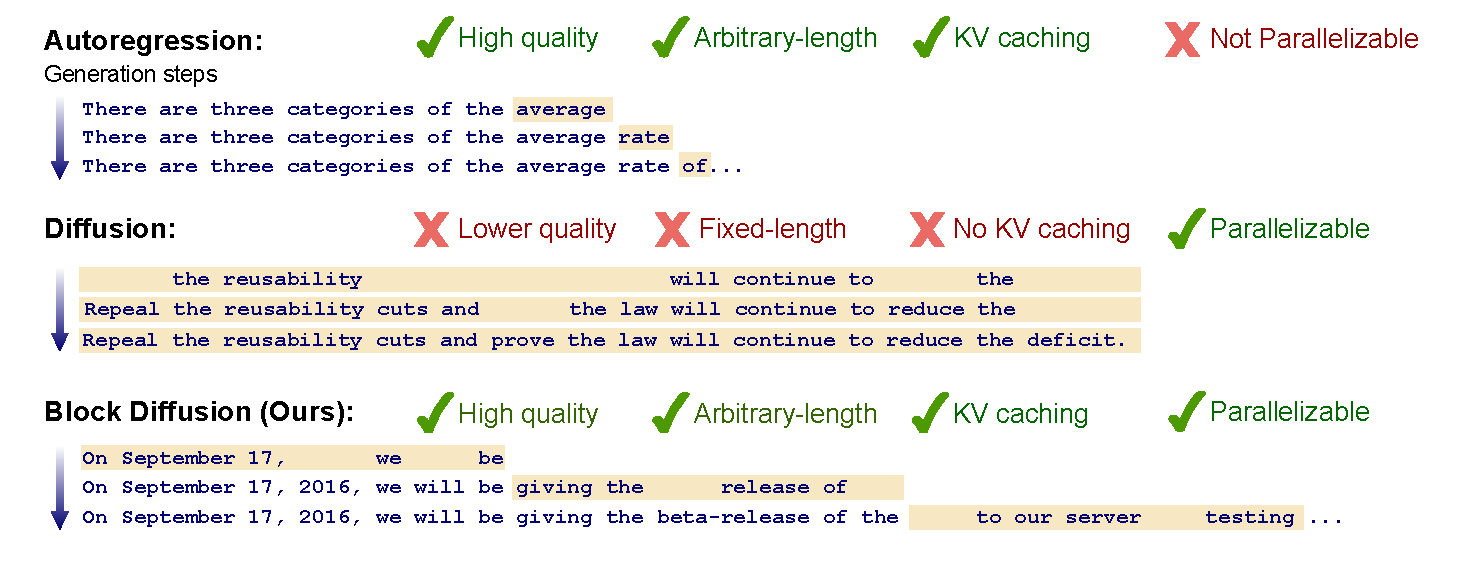
\includegraphics[width=1.1\textwidth]{figs/graphical_abstract.pdf}}
    \captionof{figure}{블록 디퓨전은 각 블록 안에서 디퓨전을 수행하고 이전 블록들에 조건화함으로써 토큰 블록을 순차적으로 생성한다. 자기회귀와 디퓨전 모델의 강점을 결합한 블록 디퓨전은 가변 길이의 더 높은 품질의 생성을 지원하고, KV 캐싱과 병렬 샘플링으로 추론 효율을 높여 두 접근의 한계를 극복한다.}
    \label{figs/graphical-abstract}
    \vspace{-5pt}
\end{figure}

% \begin{figure}
%     \centering
%     \includegraphics[width=\linewidth]{figs/graphical_abstract_v2.pdf}
%     \caption{Block diffusion models blocks of tokens autoregressively and performs diffusion within each block. By combining strength from autoregressive and diffusion models, block diffusion overcomes the limitations of both approaches by supporting arbitrary-length, higher-quality generation and faster inference with KV-caching and parallel sampling.}
%     \label{fig:graphical-abstract}
% \end{figure}


언어모델링 벤치마크에서 \algos{}를 평가하여, 학습 문맥 길이를 초과하는 길이를 포함해 임의 길이의 시퀀스를 생성할 수 있음을 시연한다. 또한 \algos{}는 이산 디퓨전 모델 가운데 새로운 최첨단 perplexity를 달성한다. %, 자기회귀 모델과의 격차를 줄이는 방향으로 진전을 이룬다.
임베딩에 대한 가우시안 디퓨전을 수행하는 다른 반자기회귀 정식화 \citep{han2022ssd,han2023ssd2}와 비교해, 우리의 이산 접근은 다루기 쉬운 가능도 추정치를 제공하고, 한 자릿수 더 적은 생성 단계로 향상된 생성 perplexity의 샘플을 만들어 낸다.
% 반자기회귀 디퓨전 모델은 또한 추론 시 여러 토큰에 걸쳐 정방향 패스를 구현할 수 있어 자연스러운 속도 이점도 가진다. 이 모델들이 자기회귀 모델로는 닿을 수 없는 파레토 경계 위의 품질-속도 절충점을 달성함을 보인다.
요약하자면, 본 연구의 기여는 다음과 같다.
\begin{itemize}
    % \item 토큰 블록 단위로 자기회귀이며 각 블록의 조건부는 이산 디퓨전을 따르는 \algofull{} (\algos{})을 도입한다. 기존 디퓨전 언어모델과 달리, \algos{}는 가변 길이 생성과 KV 캐싱을 지원한다.
    \item 토큰 블록 단위로 자기회귀이며 각 블록의 조건부가 이산 디퓨전에 기반한 블록 이산 디퓨전 언어모델을 도입한다. 기존 디퓨전 모델과 달리, 블록 디퓨전은 가변 길이 생성과 KV 캐싱을 지원한다.
    \item 모델에 입력된 토큰 배치 전체를 효율적으로 활용할 수 있게 하는, 블록 디퓨전 모델 전용 학습 알고리즘을 도입한다.
    \item 디퓨전 모델 성능의 제약 요인으로 경사 분산을 식별하고, 경사 분산을 줄이는 맞춤 데이터 주도 노이즈 스케줄을 제안한다.
    \item 본 연구의 결과는 이산 디퓨전의 새로운 최첨단 perplexity를 확립하며, 자기회귀 모델과의 격차를 줄이는 방향으로 진전을 이룬다.
\end{itemize}

%However, existing work has not shown its potential for likelihood modeling on standard benchmarks and have been limited to continuous diffusion models.
%We introduce a class of Precise Discrete Diffusion Language Models (\algos{}) that use a semi-autoregressive modeling framework and low-variance gradient estimators to close the likelihood gap with AR models.

%\algos{} achieve up to \TODO{...x} better perplexity relative to existing diffusion LMs and are within \TODO{...\%} of the autoregressive perplexity for block lengths \TODO{$L' \leq ...$}. Our analysis shows that the sample quality of \algos{} improves as $L' \rightarrow 1$ and the sample efficiency improves as $L' \rightarrow L$, which we analyze under unconditional generation and text summarization tasks.

%Our contributions are as follows:
%\begin{enumerate}
%\item We propose a semi-autoregressive (SAR) training recipe that strikes a balance between better likelihoods and faster inference by combining the strength of diffusion and autoregressive modeling
%\item We develop an efficient attention algorithm that predicts multiple tokens in parallel while supporting KV caching
%\item We introduce tunable noise schedules that further reduce the perplexity gap with autoregressive models by minimizing the variance of gradient updates during training
%\end{enumerate}

\section{배경: 언어모델링 패러다임}\label{sec:background}
\paragraph{표기법}
$V$개의 범주를 가지는 스칼라 이산 확률변수를, 단순체(simplex) $\Delta^V$의 부분집합인 공간 $\mathcal{V} = \{\x \in \{0, 1\}^{V} : \sum_i \x_i = 1\}\subset \Delta^V$ 위의 ``원-핫(one-hot)'' 열벡터로 본다. $V$번째 범주는 특수 [MASK] 토큰을 나타내며, $\m \in \mathcal{V}$는 그 원-핫 벡터이다.
$\seqx$를 $L$개의 토큰 시퀀스로 정의하며, 모든 토큰 $\ell \in \{1, \ldots, L\}$에 대해 $\x^\ell \in \mathcal{V}$이고, 그러한 모든 시퀀스의 집합을 $\mathcal{V}^L$로 표기한다. 본 논문 전반에서 표기를 단순화하여 토큰 시퀀스를 $\x$, 개별 토큰을 $\x^\ell$로 부른다. 끝으로, $\cat(\cdot; p)$를 확률 $p \in \Delta^V$인 범주 분포(categorical distribution)로 둔다.
% \begin{enumerate}
%     \item Consider a sequence of $L$ tokens $\x = \left[ x^1, \dots, x^L \right]$ drawn from the data distribution $q(\mathbf{x})$. We aim to estimate the joint probability $p(\x)$. We compare two dominant language modeling frameworks: autoregressive and diffusion LMs.
% \end{enumerate}
\subsection{자기회귀 모델}
데이터 분포 $q(\x)$에서 추출된 $L$개의 토큰 시퀀스 $\x = \left[ \x^1, \dots, \x^L \right]$를 고려하자.
% 데이터 분포 $q(\mathbf{x})$에서 추출된 $L$개의 토큰 시퀀스 $\x = \left( x^1, \dots, x^L \right)$를 고려한다. 우리의 목표는 $q$의 모델 $p_\theta(\x)$를 적합시키는 것이다.
% 두 가지 주요 언어모델링 프레임워크인 자기회귀 LM과 디퓨전 LM을 비교한다.
자기회귀(autoregressive, AR) 모델은 다음 형태로 인수분해된 분포를 정의한다.
\begin{align}\label{eq:ar-nll}
    \log p_\theta(\x) = \sum_{\ell=1}^L \log p_\theta(\xl \mid \x^{<\ell}),
\end{align}
여기서 각 $p_\theta(\xl \mid \x^{<\ell})$은 신경망으로 직접 매개변수화된다.
따라서 AR 모델은 다음 토큰 예측(next token prediction)을 통해 효율적으로 학습될 수 있다. 그러나 순차 의존성 때문에 AR 모델은 $L$개의 토큰을 생성하는 데 $L$ 단계가 필요하다.

\subsection{이산 디노이징 디퓨전 확률 모델}
% \begin{enumerate}
%     \item Diffusion models learn $p(\mathbf{x})$ by iteratively undoing a forward corruption process $q(\mathbf{x})$. Whereas AR models optimize the true likelihood, diffusion models optimize a likelihood bound. 
%     \item Discrete diffusion models, such as D3PM \citep{austin2021structured}, define the diffusion process over discrete structures using a Markov forward process $q(\x_t | \x_{t-1}) = \cat( \x_t ; Q_t \x_{t-1})$. Masked diffusion language models are a class of discrete diffusion models that set the prior distribution to a "masked" state: $\boldsymbol{\pi} = \m$ \vkl{need less content on this than in MDLM, could even drop this bullet point} \TODO{introduce diffusion in the general D3PM formulation}
%     \item MDLM \citep{sahoo2023backpropagation} tightens the ELBO of this class of diffusion LMs and achieves state-of-the-art likelihoods among diffusion models  \TODO{use interpolating noise schedule from MDLM. Define $\alpha_t$ and other relevant notation. 1-2 sentences acknowledging the ELBO, call it $\mathcal{L}(\x, \theta)$}
    
% \end{enumerate}


% Diffusion models fit a model $p_\theta(\mathbf{x})$ to undo a forward corruption process $q$ \citep{sohl2015deep,ho2020denoising,sahoo2024diffusion}. This process starts with clean data $\x$ drawn from the data distribution $q(\x)$ and defines latent variables $\x_t$ for $t \in [0, 1]$  that represent progressively noisy versions of $\x$. In the discrete-time setting, 
% % the discrete denoising diffusion probabilistic modeling (D3PM) framework 
% the D3PM framework \citep{austin2021structured}
% defines $q$ to be a  Markov forward process $q(\x_t \mid \x_{t-1}) = \cat( \x_t ; Q_t \x_{t-1})$ where $Q_t \in \mathbb{R}^{V \times V}$  is the diffusion matrix. The $Q_t$ can encode masking, random token changes, related word substitutions, and more.
% % This process induces marginals
% % \begin{equation} \label{eq:d3pm_maginal}
% %     q(\x_t | \x) = \cat(\x_t ; \bar Q_t \x)  = \cat(\x_t ; Q_t \cdot Q_{t-1} \cdots Q_1 \x).
% % \end{equation}

% An ideal diffusion model $p_\theta$ is the reverse of the process $q$. The D3PM framework defines $p_\theta$ as 
% % the mean-parameterization is only insufficient for continuous distributions. we can use simple probability here because exact marginalization is tractable.
% %\begin{align}\label{eqn:diffusion}
% %    p_\theta(\x_s | \x_t) = q(\x_s | \x_t, \x_\theta(\x_t)) & \text{ where} & q(\x_s | \x_t, \x) = \cat(\x_s ; (Q_t \x \cdot \bar Q_{t-1} \x)/(\x_t^\top \bar Q_t \x))
% %\end{align}
% \begin{align}\label{eqn:diffusion}
%     p_\theta(\x_s \mid \x_t) = \sum_{\x}q(\x_s \mid \x_t, \x)p_\theta(\x\mid \x_t),
% \end{align}
% where the denoising base model $p_\theta(\x\mid\x_t)$ predicts clean tokens $\x$ given noised tokens $\x_t$.
% The marginalization is tractable due to the independent noising process over tokens in $q$, as well as the independence assumptions commonly made in the base model: the clean tokens are modeled independently as $\prod_i p(x^i\mid \x_t)$.
% %The posterior $q(\x_s | \x_t, \x)$ has an analytical form, but involves clean data $\x$, which is unavailable at generation time. Thus, D3PM introduces a model $\x_\theta(\x_t)$ of the clean data given noisy input $\x_t$.

% An ideal diffusion model $p_\theta$ is the reverse of the process $q$. The D3PM framework defines this model as $p_\theta(\x_s | \x_t)$ based on the posterior $q(\x_s | \x_t, \x) = \cat(\x_s ; (Q_t \x \cdot \bar Q_{t-1} \x)/(\x_t^\top \bar Q_t \x))$. Since the true data $\x$ is unavailable at generation time, D3PM introduces a model $\x_\theta(\x_t)$ of the clean data given noisy input $\x_t$ and defines $p_\theta(\x_s | \x_t) = q(\x_s | \x_t, \x_\theta(\x_t))$.

% % The parameterized reverse diffusion model $p_\theta$ over $\x$ and $\x_t$ is trained to maximize a variational lower bound on log-likelihood (ELBO).
% The diffusion model $p_\theta$ is trained using variational inference.
% Given a number of discretization steps $T,$ defining $s(j) = (j -1)/T$ and $ t(j) = j /T$, and using $\KL[\cdot]$ to denote the Kullback–Leibler divergence,
% % the Markov assumption on the forward and reverse processes allows us to express this ELBO as follows \citep{sohl2015deep}
% the Negative ELBO (NELBO) equals~\citep{sohl2015deep}:
% {\footnotesize
% \begin{align}\label{eqn:elbo}
%     % &\log p_\theta(\x) \geq \mathrm{ELBO}(p_\theta, q) \\ 
%     \mathcal{L}(\x) = \E_q\Bigg[- \log p_\theta(
%     \x | \x_{t(0)}) + \sum_{j=1}^T \KL[q(\x_{s(j)} | \x_{t(j)}, \x) \| p_\theta(\x_{s(j)} | \x_{t(j)})]
%     + \KL[q(\x_{t(T)} | \x) \| p_\theta(\x_{t(T)})] \Bigg]
% \end{align}
% }

% For brevity, we drop $j$ from $t(j)$ and $s(j)$ below; in general, $s$ will denote the time step before $t$.
% This formalism extends to continuous time via Markov chain (CTMC) theory, and admits score-based generalizations \citep{song2019generative, lou2024discrete, sun2022score} and simplifications \citep{sahoo2024simple, shi2024simplified, ou2025your} that tighten the ELBO and improve performance.
% % MDLM \citep{sahoo2024simple} tightens the ELBO of this class of diffusion LMs and achieves state-of-the-art likelihoods among diffusion models.

% NEW
디퓨전 모델은 정방향 손상 과정 $q$를 역행하도록 모델 $p_\theta(\mathbf{x})$를 적합시킨다 \citep{sohl2015deep,ho2020denoising,sahoo2024diffusion}. 이 과정은 깨끗한 데이터 $\mathbf{x}$에서 시작하여, $\mathbf{x}$의 점점 더 노이즈가 많은 버전을 나타내는 잠재변수 $\mathbf{x}_t = \left[\mathbf{x}^1_t, \dots, \mathbf{x}^L_t\right]$를 $t \in [0, 1]$에 대해 정의한다. $T$ 단계로 이산화하면, $s(j) = (j -1)/T$, $t(j) = j /T$로 정의한다. 간결성을 위해 이하에서는 $t(j)$와 $s(j)$의 $j$를 생략한다. 일반적으로 $s$는 $t$ 직전의 시간 단계를 나타낸다.

D3PM 프레임워크 \citep{austin2021structured}는 $q$를 각 토큰 $\mathbf{x}^\ell$에 대해 독립적으로 작용하는 마르코프 정방향 과정으로 정의한다.
$q(\mathbf{x}^\ell_{t} \mid \mathbf{x}^\ell_{s}) = \operatorname{Cat}(\mathbf{x}^\ell_t ; Q_t \mathbf{x}^\ell_{s})$
여기서 $Q_t \in \mathbb{R}^{V \times V}$는 디퓨전 행렬이다. 행렬 $Q_t$는 마스킹, 무작위 토큰 변경, 관련 단어 치환 등 다양한 변환을 모델링할 수 있다.

% 역 사후 $q(\mathbf{x}^\ell_s \mid \mathbf{x}^\ell_t, \mathbf{x})$는 \supp{supp:elbo}에서 \citet{austin2021structured}을 따라 정의한다. 추론 시 $\x$를 사용할 수 없으므로, D3PM 프레임워크에 따라 파라미터 $\theta$의 신경망으로 매개변수화된 $\p: \mathcal{V} \times [0, 1] \to \Delta^K$로 이를 근사한다.
이상적인 디퓨전 모델 $\p$는 과정 $q$의 역과정이다. D3PM 프레임워크는 $\p$를 다음과 같이 정의한다.
\begin{align}\label{eqn:diffusion}
    p_\theta(\x_s \mid \x_t) = \prod_{\ell=1}^L p_\theta(\xl_s \mid \x_t) = \sum_{\x} \left[\prod_{\ell=1}^L q(\xl_s \mid \xl_t, \xl) p_\theta(\xl \mid \x_t)\right],
\end{align}
여기서 디노이징 기반 모델 $\p(\xl \mid \x_t)$는 노이즈 시퀀스 $\mathbf{x}_t$가 주어졌을 때 깨끗한 토큰 $\xl$을 예측하며, 역 사후 $q(\mathbf{x}^\ell_s \mid \mathbf{x}^\ell_t, \mathbf{x})$은 \citet{austin2021structured}을 따라 \supp{supp:elbo}에 정의되어 있다.
% $q$에서 토큰별 노이즈 과정이 독립이고, 기반 모델에서도 통상적으로 독립 가정($\prod_\ell p(\xl\mid \x_t)$)을 두므로 주변화는 다루기 쉽다.

디퓨전 모델 $p_\theta$는 변분 추론(variational inference)으로 학습된다. $\operatorname{KL}[\cdot]$이 쿨백–라이블러 발산(Kullback–Leibler divergence)을 나타낸다고 하자. 그러면 음의 ELBO(NELBO)는 다음과 같이 주어진다 \citep{sohl2015deep}.
{\footnotesize
\begin{align}\label{eqn:elbo}
    % &\log p_\theta(\x) \geq \mathrm{ELBO}(p_\theta, q) \\ 
    \mathcal{L}(\x; \theta) = \E_q\Bigg[- \log p_\theta(
    \x | \x_{t(1)}) + \sum_{j=1}^T \KL[q(\x_{s(j)} | \x_{t(j)}, \x) \| p_\theta(\x_{s(j)} | \x_{t(j)})]
    + \KL[q(\x_{t(T)} | \x) \| p_\theta(\x_{t(T)})] \Bigg]
\end{align}
}
이 형식은 연속 시간 마르코프 사슬(CTMC) 이론을 통해 연속 시간으로 확장되며, 점수 기반(score-based) 일반화를 허용한다 \citep{song2019generative, lou2024discrete, sun2022score}. 추가적인 단순화 \citep{sahoo2024simple, shi2024simplified, ou2025your}는 ELBO를 더 조이고 성능을 향상시킨다.

\section{블록 디퓨전 언어모델링}
우리는 토큰 블록에 대한 자기회귀 분포를 정의하고 각 블록 내부에서 디퓨전을 수행함으로써 자기회귀와 디퓨전 모델 사이를 보간하는 \algofull{} (\algos{}) 부류를 탐구한다. 최대 가능도 추정을 위한 블록 디퓨전 목적함수와 효율적인 학습·표집 알고리즘을 제시한다. 블록 크기가 1일 때 디퓨전 목적함수는 기댓값에서는 자기회귀 가능도와 동치이지만 분산이 높다는 점을 보인다. 높은 학습 분산을 디퓨전 모델의 제약으로 식별하고, 학습 시 경사 갱신의 분산을 줄이는 데이터 주도 노이즈 스케줄을 제안한다.

% \paragraph{Notation}
% Consider a sequence of $L$ tokens $\x = \left[ x^1, \dots, x^L \right]$ drawn from the data distribution $q(\mathbf{x})$. We group tokens in $\x$ into $B$ blocks of length $L'$ with $B=B$ (we assume that $B$ is an integer). We denote each block $\x^{(b-1)L':bL'}$ from token at positions $(b-1)L'$ to $bL'$ for blocks $b \in \{ 1, \dots, B \}$ as $\x^b$ for simplicity.

\subsection{블록 디퓨전 분포와 모델 아키텍처}\label{sec:sar-elbo}
\cref{sec:background}의 언어모델링 패러다임을, 토큰 블록을 자기회귀적으로 모델링하면서 각 블록 내부에서 디퓨전을 수행하도록 결합할 것을 제안한다.
% $L$을 사전학습 시퀀스 길이로, $L'$을 각 SAR 블록의 길이로 두며 $L' < L$이라 하자.
% 따라서 로그가능도는 $L'$ 길이의 블록 시퀀스에 대해 다음과 같이 인수분해된다.
$\x$의 토큰을 길이 $L'$의 $B$개 블록으로 묶으며 $B=L/L'$이다($B$가 정수라 가정). 위치 $(b-1)L'$부터 $bL'$까지의 각 블록 $\x^{(b-1)L':bL'}$($b \in \{ 1, \dots, B \}$)을 단순히 $\x^b$로 표기한다. 우리의 가능도는 블록에 대해 다음과 같이 인수분해된다.
% where we have $B=L/L'$ blocks in the sequence. We denote each block $\x^{(b-1)L':bL'}$ from token at positions $(b-1)L'$ to $bL'$ for blocks $b \in \{ 1, \dots, B \}$ as $\x^b$ for simplicity:
\begin{align}\label{eqn:sar-ll}
     \log p_\theta(\x) &= \sum_{b = 1}^{B} \log p_\theta(\x^{b} \mid \x^{<b}),
\end{align}
그리고 각 $p_\theta(\x^b \mid \x^{<b})$는 $L'$개 토큰의 블록에 대한 이산 디퓨전으로 모델링된다.
% 구체적으로, $\x^b$에 마르코프 정방향 노이즈 과정 $q(\x_t^b|\x_s^b)$이 적용되며, 역모델 $p_\theta(\x_s^b | \x_t^b, \x^{<b}) = q(\x_s^b | \x_t^b, \x^b_\theta(\x^b_t, \x^{<b}))$은 (\ref{eqn:diffusion})처럼 정의되되 블록 $b$로 제한된다.
구체적으로, (\ref{eqn:diffusion})처럼 정의되되 블록 $b$로 제한된 역 디퓨전 과정을 정의한다.
%$p_\theta(\x_s^b | \x_t^b, \x^{<b}) = q(\x_s^b | \x_t^b, \x^b_\theta(\x^b_t, \x^{<b}))$
\begin{align}
    p_\theta(\x_s^b \mid \x_t^b, \x^{<b}) = \sum_{\x^b} q(\x_s^b \mid \x_t^b, \x^b)p_\theta(\x^b\mid \x^b_t,\x^{<b})
\end{align}
%Note that since each $p_\theta(\x^{b} \mid \x^{<b})$ is a distribution over $\x^{b} $ conditioned on $\x^{<b}$, the model $\x_\theta$ which denoises $\x^b_t$ is also conditioned on $\x^{<b}$.
(\ref{eqn:sar-ll})의 각 항에 (\ref{eqn:elbo})의 NELBO를 적용하여 다음과 같은 원칙적인 학습 목적함수를 얻는다.
\begin{align}\label{eqn:sar-elbo}
    - \log p_\theta(\x) \leq \mathcal{L}_\text{BD}(\x; \theta) := \sum_{b=1}^{B} \mathcal{L}(\x^b, \x^{<b}; \theta),
\end{align}
여기서 각 $\mathcal{L}(\x^b, \x^{<b}; \theta)$는 $\log p_\theta(\x^{b} \mid \x^{<b})$에 적용한 (\ref{eqn:elbo})의 한 사례이다. 모델이 $\x^{<b}$에 조건화되므로, $\mathcal{L}$에서 $\x^{<b}, \theta$에 대한 의존을 명시한다.
이 항들의 합을 $\mathcal{L}_\text{BD}(\x; \theta)$로 표기한다(그 자체로 유효한 NELBO이다).

% \marianne{We note that "block diffusion" modeling is synonymous with "}
% We adopt the simplified objective from \cite{sahoo2024simple} (the full derivation is provided in Suppl. \ref{supp:elbo}):
% \begin{align}\label{eqn:sar-elbo}
%     \mathcal{L}(\x, \theta) \geq \sum_{b=1}^{L/L'} \mathbb{E}_{t \sim [0, 1]} \mathbb{E}_{q} \frac{1}{1-\at} \log
%     \langle p_\theta(\x^b | \x_t^b, \x^{<b}), \x^b \rangle
% \end{align}
% The ELBO is tight for $B=1$ but becomes a looser approximation of the true log-likelihood for $B \rightarrow L$  (see Suppl. \ref{supp:sar-elbo-tightness}).

\paragraph{모델 아키텍처}
% 신경망에 대해 이상적으로는 f_\theta를 사용
결정적으로, $B$개의 기반 디노이저 모델 $p_\theta(\x^b \mid \x^b_t, \x^{<b})$를 단일 신경망 $\x_\theta$로 매개변수화한다. 신경망 $\x_\theta$는 확률 $p_\theta(\x^b \mid \x_t^b, \x^{<b})$뿐 아니라 효율적인 학습을 위한 계산 산출물도 출력한다. 이는 모든 $B$개 블록에 대한 손실 $\mathcal{L}_\text{BD}(\x; \theta)$를 메모리 효율적으로 병렬 계산할 수 있게 해 준다.
구체적으로, 블록-인과(block-causal) 어텐션 마스크를 사용하는 트랜스포머 \citep{vaswani2017attention}로 $\x_\theta$를 매개변수화한다. 트랜스포머 $\x_\theta$는 $L$개 토큰에 적용되며, 블록 $b$의 토큰들은 블록 1부터 $b$까지의 토큰들에만 주의를 기울인다. $\x_\theta$가 학습되면, $\x^b_\theta(\x^b_t, \x^{<b})$는 노이즈 $\x^b_t$와 깨끗한 $\x^{<b}$를 바탕으로 블록 $b$ 안 디노이즈된 토큰에 대한 $L'$개의 예측을 만들어 낸다. % 이전 블록들로부터.

자기회귀 생성에서는 이전에 생성된 토큰의 키와 값을 캐싱해 매 단계 재계산을 피하는 것이 일반적이다. 마찬가지로, 블록 $b$의 키와 값을 $\mathbf{K}^b, \mathbf{V}^b$로 표기하고, $\x_\theta$가 이를 입력·출력으로 지원하도록 정의한다. $\x_\theta$의 전체 시그니처는 다음과 같다.
\begin{align}\label{eqn:model-kv}
    \x_\text{logits}^b, \mathbf{K}^b, \mathbf{V}^b \gets \x^b_\theta(\x^b_t, \mathbf{K}^{1:b-1}, \mathbf{V}^{1:b-1}) := \x^b_\theta(\x^b_t, \x^{<b}),
\end{align}
여기서 $\x_\text{logits}^b$는 깨끗한 $\x^b$에 대한 예측이고, $\mathbf{K}^b, \mathbf{V}^b$는 $\x_\theta$의 정방향 패스에서 만들어진 키-값 캐시이며, $\mathbf{K}^{1:b-1}, \mathbf{V}^{1:b-1}$은 $\x^{<b}$에 대한 $\x_\theta$ 정방향 패스에서 캐시된 키와 값이다(따라서 입력 $\x^{<b}$와 $\mathbf{K}^{1:b-1}, \mathbf{V}^{1:b-1}$는 동치이다).

% 실제로 (\ref{eqn:sar-elbo})의 블록 $\b \in 1, \dots, B$에 대해 $p_\theta(\x^b |\x_t^b, \x^{<b})$를 트랜스포머 아키텍처로 매개변수화한다. 백본은 노이즈 블록 $\x^b_{t_b} \sim q_{t_b}(\cdot|\x^b)$와 이전 블록의 깨끗한 토큰 $\x^{<b}$를 입력으로 받아 logits $\x_{\text{logit}} \gets \x_\theta^b(\x_{t_b}^b, \x^{<b})$를 만든다.


\subsection{효율적 학습·표집 알고리즘}\label{sec:eff-algs}

이상적으로는 손실 $\mathcal{L}_\text{BD}(\x; \theta)$를 $\x_\theta$의 한 번의 정방향 패스로 계산하고 싶다. 그러나 $\x_t^b$를 디노이징하려면 이 노이즈 입력에 대한 정방향 패스가 필요하고, 다음 블록을 디노이징하려면 $\x_\theta$를 깨끗한 버전 $\x^b$에 대해 실행해야 한다. 따라서 모든 블록은 모델을 최소 두 번 통과해야 한다.

\paragraph{학습}
이 관찰을 바탕으로, 위의 최소 계산 요구를 가진 학습 알고리즘을 제안한다
%
% 그러나 $\x_{t_b}^b$의 쿼리 $Q^b$가 이전 블록 $\x^{<b}$의 키·값 $\mathbf{K}^{1:b\text{-}1}, \mathbf{V}^{1:b\text{-}1}$에 주의해야 하므로, 고전적인 트랜스포머 신경망의 일반적인 정방향 패스로는 이를 할 수 없다.
% 우리는 이를 맞춤 학습 알고리즘으로 수행하기를 제안한다
(Alg.~\ref{alg:sar-train}). 구체적으로, 첫 번째 정방향 패스 $(\emptyset, \mathbf{K}^{1:B}, \mathbf{V}^{1:B}) \gets \x_\theta(\x)$에서 전체 시퀀스 $\x$의 키와 값 $\mathbf{K}^{1:B}, \mathbf{V}^{1:B}$를 미리 계산한다.
그런 다음 모든 블록에 대한 디노이즈 예측을 $\x_\theta^b(\x_{t}^b,  \mathbf{K}^{1:b\text{-}1}, \mathbf{V}^{1:b\text{-}1})$로 계산한다. 각 토큰은 $\x_\theta$를 두 번 통과한다.

\paragraph{벡터화 학습}

단순한 방법으로는 $\x_\theta^b(\x_{t}^b,  \mathbf{K}^{1:b\text{-}1}, \mathbf{V}^{1:b\text{-}1})$를 $B$번 반복 적용해 logits를 계산할 것이다. 우리는 깨끗한 데이터 $\x$와, 각 블록 $\x^b$에 노이즈 수준 $t_b$를 적용해 얻은 노이즈 데이터 $\x_\text{noisy} = \x^1_{t_1} \oplus \dots \oplus \x^B_{t_B}$의 결합 $\x_\text{noisy} \oplus \x$에 대해 한 번의 정방향 패스로 $\mathcal{L}_\text{BD}(\x; \theta)$를 계산하는 벡터화 구현을 제안한다. 노이즈 토큰들이 같은 블록 안 다른 노이즈 토큰들과 이전 블록 안 모든 깨끗한 토큰들에 주의를 기울이도록 $\x_\text{noisy} \oplus \x$에 대한 어텐션 마스크를 설계한다(\supp{suppl:masks} 참조). 본 방법은 \algos{} 학습의 오버헤드를 다루기 좋게 유지하며, 사전학습과 결합해 비용을 더 줄인다.
% In practice, this procedure is about 50\% slower than diffusion training. 

% As a result, we efficiently model the conditional likelihoods between blocks relative to a naive implementation that requires $B$ forward passes for each conditional term. We may do so using two forward passes (one for pre-computing keys and values $\mathbf{K}^{1:B}, \mathbf{V}^{1:B}$ and the second for computing logits $\x_{\text{logit}}$), or through a single forward pass on $\x_t \oplus \x$ using a custom mask to mimic the proposed attention pattern (more details in Suppl. \ref{suppl:masks}).


\paragraph{표집} 한 번에 한 블록씩 이전에 표집된 블록들에 조건화하여 표집한다(Alg.~\ref{alg:sar-inference}). 조건부 분포 $p_\theta(\x_{s}^b | \x_{t}^b, \x^{<b})$로부터 표집하기 위해 어떤 표집 절차 $ \textsc{Sample}(\x_\theta^b, \mathbf{K}^{1:b\text{-}1},\mathbf{V}^{1:b\text{-}1})$이든 사용할 수 있으며, 문맥 조건화는 미리 계산된 키와 값 $\mathbf{K}^{1:b-1}, \mathbf{V}^{1:b-1}$을 활용한 크로스 어텐션으로 생성된다. AR 모델처럼, 새 블록을 표집할 때 키와 값을 다시 계산하지 않고 캐싱하면 계산을 절약할 수 있다.

특히 우리의 블록 디퓨전 디코딩 알고리즘은 임의 길이의 시퀀스를 표집할 수 있게 해 주는 반면, (일반) 디퓨전 모델은 고정 길이 생성으로 제한된다. 또한 우리의 샘플러는 각 블록 안에서 병렬 생성을 허용하지만, AR 샘플러는 토큰 단위 생성으로 제한된다.

\input{algs/short_algs}


\section{디퓨전과 AR 모델 사이 가능도 격차의 이해}

% \subsection{\algofull{} (\algos{})}
\subsection{마스크 \algos{}}

가장 효과적인 디퓨전 언어모델은 토큰이 점진적으로 특수 마스크 토큰으로 치환되는 마스킹 노이즈 과정을 활용한다 \citep{austin2021structured,lou2024discrete,sahoo2024simple}. 여기서는 마스크 디퓨전 언어모델링 프레임워크 \citep{sahoo2024simple, shi2024simplified, ou2025your}에 기반한 블록 디퓨전 모델의 특수 부류인 마스크 \algos{}를 도입한다.

보다 형식적으로, 토큰 $\ell \in \{1, \dots, L\}$에 대해 토큰별 노이즈 과정 $q(\xl_t| \xl) = \cat(\xl_t; \at \xl + (1 - \at) \m)$을 채택한다. 여기서 $\m$은 마스크 토큰의 원-핫 인코딩이고, $\alpha_t \in [0, 1]$은 $\alpha_{0} = 1$, $\alpha_{1} = 0$을 만족하는 $t$에 대한 엄격히 감소 함수이다. 시간 $t$에서 토큰이 마스킹될 확률이 $1-\alpha_t$인 선형 스케줄을 사용한다.
\cite{sahoo2024simple, shi2024simplified, ou2025your}의 단순화된 목적함수를 채택한다(전체 유도는 \supp{supp:elbo}에 있다).
\begin{align}\label{eqn:sar-elbo-exp}
    - \log p_\theta(\x) \leq \mathcal{L}_\text{BD}(\x; \theta) :=  \sum_{b=1}^{B} \mathbb{E}_{t \sim [0, 1]} \mathbb{E}_{q} \frac{\at'}{1-\at} \log p_\theta(\x^b | \x_{t}^b, \x^{<b})
\end{align}
\noindent 여기서 $\at'$은 $T \rightarrow \infty$로 보내는 (\ref{eqn:elbo})의 연속 시간 확장 하에서 $\at$의 순간 변화율이다. NELBO는 $L'=1$에서 타이트(tight)하지만, $L' \rightarrow L$로 갈수록 참 음의 로그가능도에 대한 더 느슨한 근사가 된다(\supp{supp:sar-elbo-tightness} 참조).

\subsection{사례 연구: 단일 토큰 생성}
\begin{wraptable}{r}{5cm}
    \small
  \vspace{-15pt}
  \caption{LM1B에서 16B 토큰에 대한 단일 토큰 생성의 테스트 perplexity(PPL; $\downarrow$).}
  \label{tab:bs1-var}
  \centering
  \begin{tabular}{lll}
    \toprule
    & PPL ($\downarrow$)  \\
    \midrule
    AR  & \textbf{22.88} \\
    \hspace{1em} + random batch size & 24.37 \\
    \midrule
    \algo{} $L'=1$ & $\leq$ 25.56\\
    \hspace{1em} + tuned schedule & \textbf{22.88} \\
    \bottomrule
  \end{tabular}
  \vspace{-10pt}
\end{wraptable}
우리의 블록 디퓨전 매개변수화 (\ref{eqn:sar-elbo-exp})은 $L'=1$의 극한에서 자기회귀 NLL (\ref{eq:ar-nll})과 기댓값에서 동치이다(\supp{supp:sar-block1-nll} 참조). 놀랍게도, LM1B 데이터셋으로 두 모델을 학습하면 $L'=1$의 블록 디퓨전 모델과 AR 사이에 perplexity 격차가 약 2 포인트 있음을 발견한다.


목적함수가 기댓값에서는 동치이지만, 남은 perplexity 격차는 높은 학습 분산의 결과임을 보인다. AR은 $L$개 토큰의 교차 엔트로피로 학습되는 반면, $L'=1$의 우리 블록 디퓨전 모델은 마스크 토큰 $\xl_t = \m \; \forall \ell \in \{ 1, \dots L \}$에 대해서만 교차 엔트로피를 계산하여 $\mathbb{E}_{t \sim \mathcal{U}[0,1]} q(\xl_t = \m | \xl) = 0.5$가 된다. 따라서 디퓨전 목적함수로 학습하면 손실 경사를 2배 더 적은 토큰으로 추정하게 되어 AR 대비 학습 분산이 커진다.

가능도 격차를 닫기 위해, 정방향 과정을 토큰을 완전히 마스킹하도록(즉, $q(\xl_t = \m | \xl) =1$) 설계하여 $L'=1$인 \algo{}를 학습한다. 이 스케줄에서 디퓨전 목적함수는 AR 목적함수와 \textit{동치}가 된다(\supp{supp:sar-block1-nll}). 표 \ref{tab:bs1-var}에서, 블록 디퓨전 목적함수로 학습한 결과 perplexity가 AR 학습과 같음을 보인다. 경험적으로 이는 그림 \ref{figs/bs-1}처럼 학습 손실의 분산을 줄여 준다. 노이즈 스케줄 튜닝이 목적함수의 분산을 줄임을 328M 토큰 학습 후 $\text{Var}_{\x, t} \left[ \mathcal{L}_{\text{BD}} (\x; \theta)\right]$를 측정하여 검증한다. NELBO로 학습하면 분산이 1.52인 반면, 완전 마스킹 학습으로는 분산이 0.11로 감소한다.
\begin{figure}
\centering
    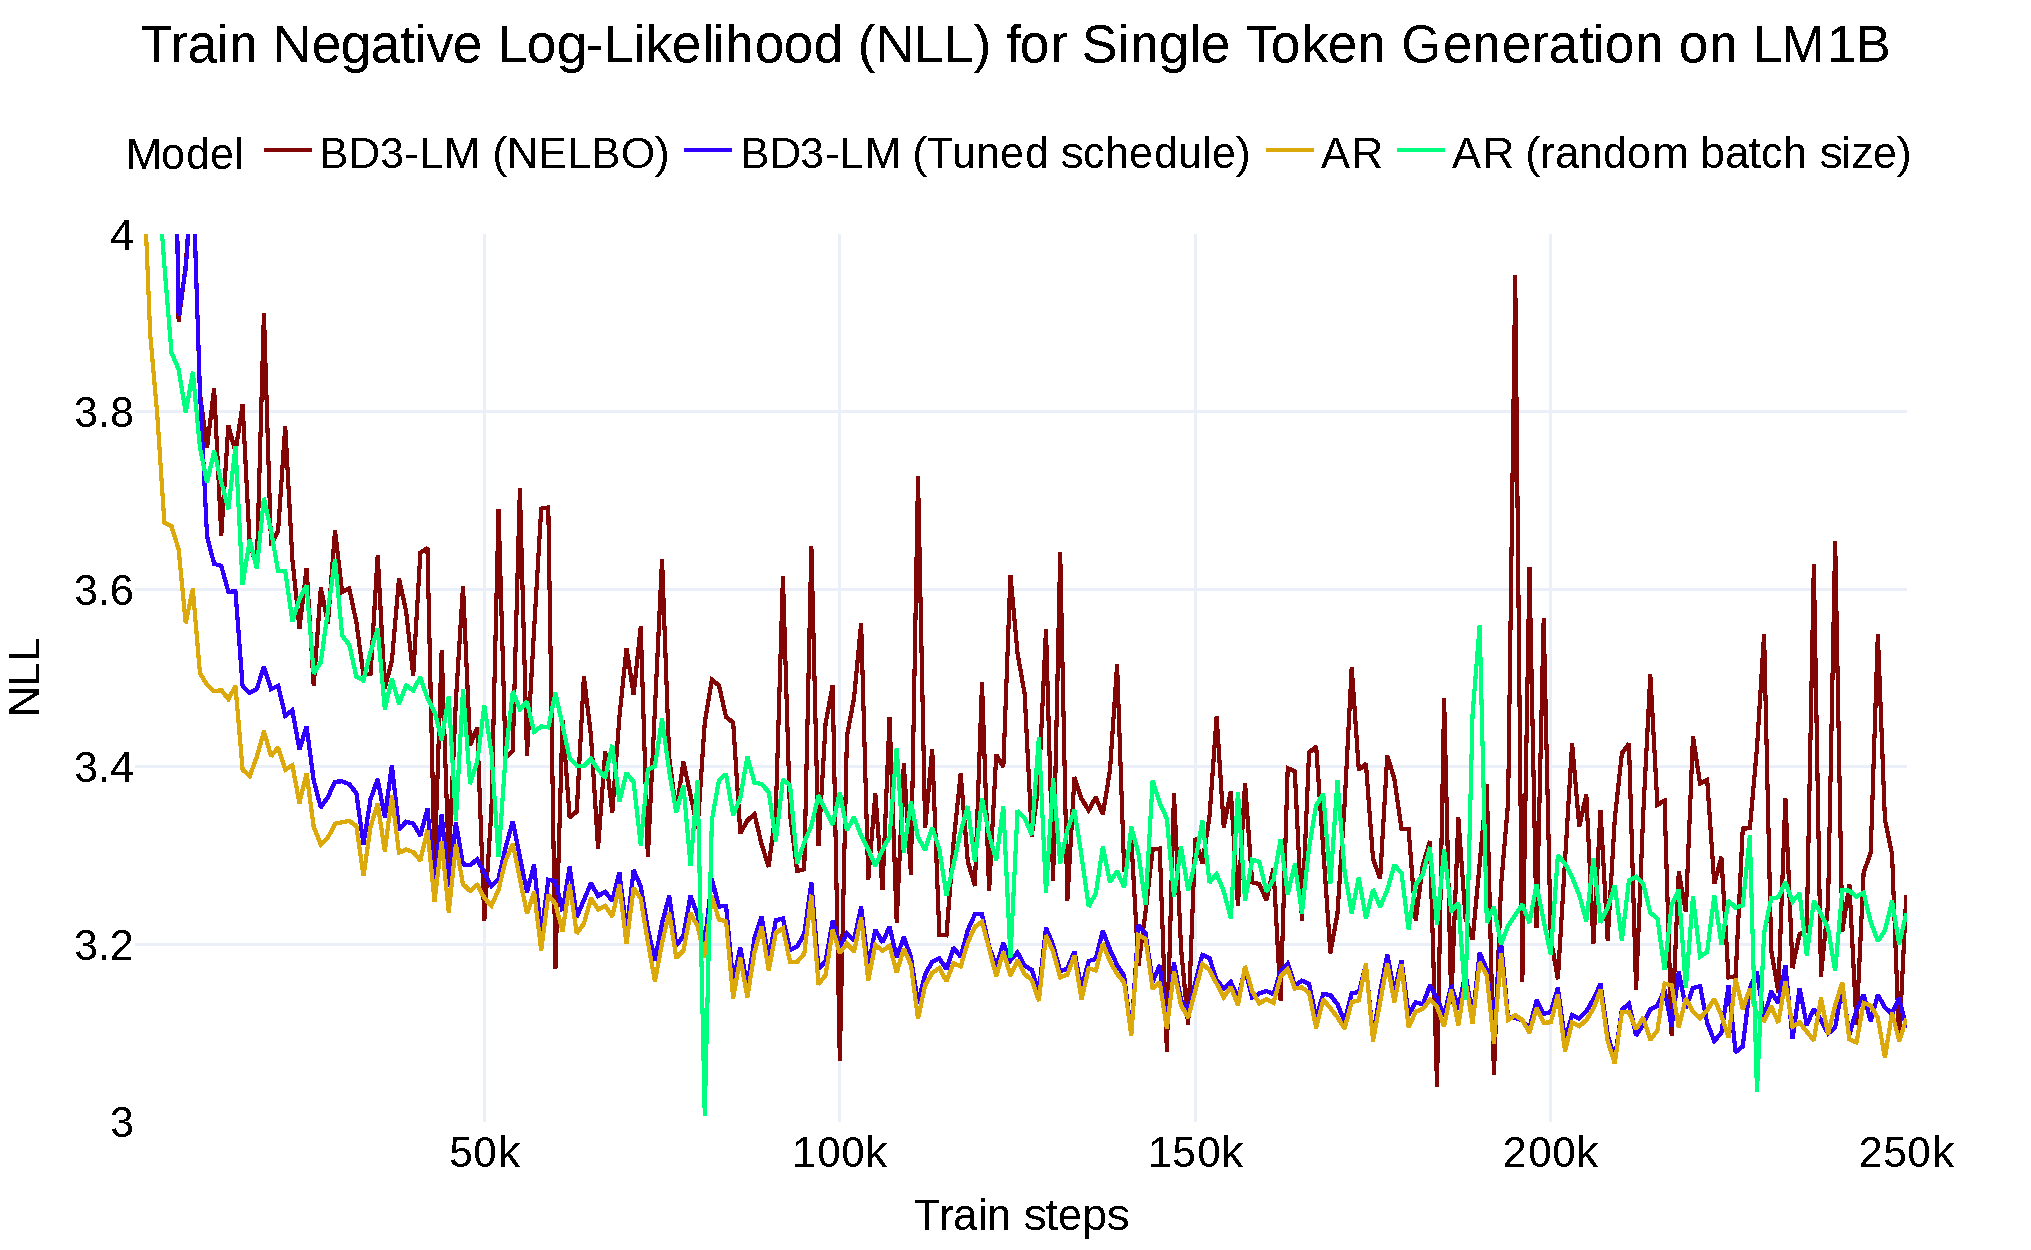
\includegraphics[width=0.75\textwidth]{figs/bs1.pdf}
    \captionof{figure}{LM1B에서 토큰별 가능도 모델링의 학습 NLL. 모델은 16B 토큰으로 학습된다. 배치 안 토큰의 평균 절반이 마스킹되는 이산 디퓨전 NELBO로 학습할 때, 무작위 배치 크기를 가진 AR 모델과 비슷한 학습 분산을 가진다.}
    \label{figs/bs-1}
\end{figure}


\subsection{높은 분산 학습이 만드는 디퓨전 격차}
다음으로, 디퓨전 모델 학습에서 경사 분산 문제를 형식적으로 기술한다. 단일 토큰 생성에 대한 경험적 관찰을 바탕으로, $L' \geq 1$의 디퓨전 모델 학습 분산을 최소화하기 위해 사용할 경사 분산 추정량을 제안한다. NELBO는 노이즈 스케줄 선택에 불변이지만(\supp{supp:elbo}), 이 불변성은 학습 시 사용하는 손실의 몬테카를로(Monte Carlo) 추정량에는 성립하지 않는다. %$\x \sim q_0, t \sim \mathcal{U}[0, 1]$, $\x_t \sim q_t(\x)$의 표집에 대해.
따라서 추정량과 그 경사의 분산은 스케줄에 의존한다. 먼저 배치 크기 $K$에서의 NELBO 추정량을 표현한다. %$l_\theta (\x)$
시퀀스 배치를 $\mathbf{X} = \left[\x^{(1)}, \x^{(2)}, \ldots, \x^{(K)}\right]$로 표기하고, 각 $\x^{(k)}\overset{\text{iid}}\sim q(\x)$이다. 배치 NELBO 추정량은 아래와 같으며, $t(k, b)$는 시퀀스 $k$와 블록 $b$에서 표집된다.
\begin{align}
\mathcal{L}_\text{BD}(\mathbf{X}; \theta)
:= l(\mathbf{X}; \theta)
= \frac{1}{K} \sum_{k=1}^K \sum_{b=1}^B  \frac{\alpha_{t(k, b)}'}{1-\alpha_{t(k,b)}}
\log p_\theta \left(
    \x^{(k),b} \mid \x_{t(k,b)}^{(k),b}, \x^{(k), <b}
\right)
\end{align}
% We derive a Monte Carlo estimator of the diffusion ELBO over batch size $K$ and $B$ blocks:
% \begin{align}\label{eq:estimator}
%    \mathcal{L}_{[0, 1]}(\theta ; \mathbf{X}) &= \mathbb{E}_{\x \sim q_0} \sum_{b=1}^{B}  \mathbb{E}_{t \sim [0, 1]} \mathbb{E}_{q} \frac{1}{1 - \at} \log \langle p_\theta(\x_t^b | \x^{<b}), \x^b \rangle \\
%    &\approx \frac{1}{K} \sum_{k=1}^K \sum_{b=1}^B  \frac{1}{1-\alpha_{t_b}} \log \langle p_\theta(\x_{t_b}^{k, b} | \x^{k, <b}), \x^{k, b} \rangle 
% \end{align}
% \vkl{may want to briefly define the new variables}



% \begin{align}
%     \nabla_\theta \mathbb{E}_{\x \sim q(\x)} [\mathcal{L}_\text{MDLM}(\x)] &\approx  \hat{g}_{[0,1]} = \frac{1}{K} \sum_{k=1}^K \sum_{b=1}^B \frac{\alpha'_t}{1-\alpha_{t_{k,b}}}  \nabla_\theta \log p_\theta(\x^{k, b} \mid \x_{t_{k,b}}^{k, b}, x^{k, <b})  
% \end{align}
% \noindent where under the linear schedule $\at = 1 - t$, $\at'$ is constant across $t \in [0, 1]$.

% We now analyze the variance of the gradient estimator. For simplicity we define the gradient of the Monte Carlo loss estimate as $l_\theta$:
% % \begin{align}
% %     f_\theta (\x_t) = \nabla_\theta  \log \langle p_\theta(\x_t^b | \x^{<b}), \x^b \rangle \quad \text{and} \quad \bar{f}_\theta = \frac{1}{K} \sum_{k=1}^K\sum_{b=1}^B\sum_{i=1}^M  \frac{\alpha_t'}{1-\alpha_{t_i}} \nabla_\theta \log \langle p_\theta(\x_{t_i}^{b} | \x^{<b}), \x^{b} \rangle
% % \end{align}


각 배치 $\mathbf{X}^m \; \forall m \in \{ 1, \dots, M\}$에 대한 $M$개 배치에 걸친 경사 추정량의 분산은 다음과 같다.
 \begin{align}\label{eq:grad-var-estimator}
     \text{Var}_{\mathbf{X}, t}\left[
    \nabla_\theta l (\mathbf{X}; \theta) \right] 
&\approx  \frac{1}{M-1} \sum_{m=1}^M \left\lVert 
    \nabla_\theta l (\mathbf{X}^m; \theta) - \frac{1}{M} \sum_{m=1}^M \nabla_\theta l(\mathbf{X}^m; \theta)
\right\rVert^2_2
\end{align}
 % \vkl{small aesthetic question: you introduce $1/(1-\alpha_t)$ in (9) for one term and in (10) for the other term, is that intentional?}


%, \x_t \sim q_t(\x), \x \sim q_0$. 

%\vkl{the superscript notation is overloaded and in one formula we use k to denote a datapoints in a batch, and in the other one we use k (or $k_m$) to denote the batch itself}

% \subsubsection{Pitfalls of gradient estimation under sampling uniform mask rates}

% \vkl{I don't think we need this section anymore?}

% We observe empirically that the gradient estimator $\nabla_\theta g (\x)$ under uniformly sampling mask rates $1 - \alpha_t \sim \mathcal{U}[0, 1]$ suffers from high variance. As we saw in the case of modeling a single token, we observed high variance training that contributed to a 2 point perplexity gap on LM1B and high-variance gradient estimates.

% In Table \ref{tab:lm1b_vars}, we observe that training using uniformly sampled mask rates results in higher-variance estimates of the NLL compared to training on a subset of masking rates.

\section{\algos{}를 위한 저분산 노이즈 스케줄}
 % 위의 관찰을 이용해, 노이즈 스케줄을 제어하는 \algos{} 전용의 개선된 저분산 경사 추정량을 유도한다.

 \subsection{직관: 극단적 마스크율을 피하기}
경사 추정량의 분산을 최소화하고 학습을 가장 효율적으로 만드는 스케줄을 찾는 것이 목표이다.
%
마스크 환경에서는 무작위 수의 토큰을 마스킹하여, 모델이 다양한 수준의 노이즈를 되돌리는 법을 학습하게 하고자 한다. 이는 표집 시 중요하다.
그러나 너무 적은 토큰만 마스킹하면 재구성이 쉽고 유용한 학습 신호를 주지 못한다. 모든 것을 마스킹하면 최적 재구성은 데이터 분포에서 각 토큰의 주변(marginals)이며, 학습이 쉽지만 다시 유용하지 않다. 이러한 극단적 마스크율은 분산이 큰 나쁜 경사로 이어진다. 우리는 단순하고 효과적인 새로운 스케줄 부류로 이를 클리핑(clipping)하는 법을 학습하고자 한다.
% However, the precise optimal sampling distribution depends on the size of the block: we saw that for small blocks, we may want to mask everything, while larger blocks would benefit from smaller rate
% We attribute high-variance training to sampling extreme masking rates. Intuitively, if the mask rate $1-\alpha_t$ is too low, most tokens are unmasked the denoising task is too easy and the gradient is not useful for training. Similarly, if the masking rate is too high, then the Bayes optimal solution is to predict the marginals of the data distribution. \TODO{might be a bit too hand-wavey}

% Furthermore, our empirical analysis on the variance of our proposed gradient estimator demonstrate that sampling lighter mask rates results in high-magnitude gradients. However, for larger block sizes $L' \geq 8$, there exists a threshold where masking that is too heavy will result in low-quality logits from limited context.

% \vkl{I think we can expand more on this intuition. I think the idea is that if the mask is too high, the problem is too easy (you just predict the marginals of the data) and the gradient is not useful; if the mask \% is too low, then it's also too easy (nothing is masked) and the gradient is not useful}

\subsection{저분산 경사를 위한 클리핑 스케줄}
% 경사 추정량에서 높은 분산을 유발하는 $t$의 표집을 피해 경사 추정량의 분산을 줄인다.

마스크율 $1-\at \sim \mathcal{U}[\beta, \omega]$($0 \leq \beta, \omega \leq 1$)에서 표집하는 ``클리핑(clipped)'' 노이즈 스케줄 부류를 제안한다. 몬테카를로 경사 추정의 관점에서 이러한 스케줄은, 지정된 범위 이전에는 마스크 확률이 약 0이고($1-\alpha_{<\beta} \approx \epsilon$), 지정된 범위 이후에는 약 1인($1-\alpha_{>\omega} \approx 1-\epsilon$) 연속 스케줄과 동치임을 주장한다. 그 결과 범위 안에서는 $\at'$이 선형이다: $\at' \approx 1 / (\beta - \omega)$.
% % \vkl{this bracket notation is a bit confusing}. 
% We derive the Monte Carlo estimators of the diffusion ELBO under such clipped schedules:
% \begin{align}\label{eq:clipped-estimator}
%    \mathcal{L}_{[\beta, \omega]}(\theta ; \mathbf{X}) &\approx \frac{1}{K} \sum_{k=1}^K \sum_{b=1}^B \sum_{i=1}^M  \frac{\beta - \omega}{1-\alpha_{t_i}} \log \langle p_\theta(\x_{t_i}^b | \x^{<b}_k), \x^b_k \rangle 
% \end{align}

% \begin{align}
%     f_\theta (\x_t) = \nabla_\theta \log \langle p_\theta(\x_t^b | \x^{<b}), \x^b \rangle \quad \text{and} \quad \bar{f}_\theta = \frac{1}{K} \sum_{k=1}^K\sum_{b=1}^B \sum_{i=1}^M  \frac{\beta - \omega}{1-\alpha_{t_i}} \nabla_\theta \log \langle p_\theta(\x_{t_i} | \x^{<b}_k), \x^{b}_k \rangle
% \end{align}
% \vkl{above $f$ is not a function of $\omega, \beta$} \vkl{also many comments from previous section apply here}We propose a new gradient estimator for these schedules, $\hat{g}_{[\beta, \omega]}$. We derive the variance of the gradient estimator of our linear schedule $\hat{g}_{[\beta, \omega]}$ as where $t \sim \mathcal{U}[\beta, \omega], \x_t \sim q_t(\x), \x \sim q_0$. We propose the estimator :

%  \begin{align}\label{eq:grad-var-estimator}
%       \text{Var}_{\x, t}\left[ \nabla_\theta g \right] &=  \frac{1}{M-1} \sum_{m=1}^M \left\lVert \nabla_\theta l_\theta (\x^{m}) - \frac{1}{M} \sum_{m=1}^M \nabla_\theta l_\theta(\x^m) \right\rVert^2_2
% \end{align}

% We show that there exists $\beta, \omega$ that improves the variance of the gradient estimate: $\text{Var}_{\x, t} \left[\hat{g}_{[\beta,\omega]}\right] < \text{Var}_{\x, t} \left[\hat{g}_{[0, 1]}\right]$.
% \TODO{need a proof, can put the full proof in the appendix. just need to show that increasing the bounds increases the variance}

\subsection{블록 크기별 데이터 주도 클리핑 스케줄}\label{sec:data-driven-schedules}
최적 마스크율은 블록 크기 $L'$에 따라 다를 수 있으므로, 학습 중에 스케줄을 적응적으로 학습한다. \cite{kingma2021variational}는 제곱 디퓨전 손실로 분산 항을 분리해 분산 최소화를 수행하지만, 이 전략은 식 \ref{eq:grad-var-estimator}의 우리 분산 추정량에 직접 적용되지 않는다. 우리는 무작위 $t_b$뿐 아니라 무작위 배치 전반에서도 분산을 줄이고자 하기 때문이다.

대신, 학습 분산을 직접 최소화하도록 파라미터 $\beta, \omega$를 최적화한다. 최적화의 계산 부담을 줄이기 위해, 경사 추정량의 대리값(proxy)으로 디퓨전 ELBO 추정량의 분산을 사용해 $\beta, \omega$를 최적화한다: $\min_{\beta, \omega} \text{Var}_{\mathbf{X}, t} \left[ \mathcal{L}(\mathbf{X}; \theta, \beta, \omega) \right]$. 학습 중 정기적인 간격으로 격자 탐색(grid search)을 수행하여 최적 $\beta, \omega$를 찾는다(실험 세부 사항은 \cref{sec:experiments}).

표 \ref{tab:lm1b_vars}에서 디퓨전 NELBO의 분산이 테스트 perplexity와 상관관계가 있음을 보인다. 다양한 ``클리핑'' 노이즈율 분포 하에서, 블록 크기 $L' \in \{4, 16, 128\}$ 각각에 대해 NELBO의 분산과 테스트 perplexity를 모두 최소화하는 고유한 분포가 존재함을 확인한다.



\begin{table*}[ht]
    \small
  \caption{Perplexity(PPLs; $\downarrow$)와 NELBO 분산 $\text{Var}_{\mathbf{X}, t}\left[ \mathcal{L}_\text{BD}(\mathbf{X}; \theta)  \right]$ (Var. NELBO; $\downarrow$). 모델은 선형 스케줄로 LM1B에서 65B 토큰을 학습한 뒤 10B 토큰으로 파인튜닝된다.}
  \label{tab:lm1b_vars}
  \centering
  \setlength{\tabcolsep}{6pt} % Adjust horizontal padding
  \renewcommand{\arraystretch}{1.1} % Adjust vertical space between rows
  \begin{tabular}{ccccccccc}
    \toprule
     & \multicolumn{2}{c}{$\mathcal{U}[0, .5]$} & \multicolumn{2}{c}{$\mathcal{U}[.3, .8]$} & \multicolumn{2}{c}{$\mathcal{U}[.5, 1]$} & \multicolumn{2}{c}{$\mathcal{U}[0, 1]$}  \\
    \cmidrule(lr){2-3} \cmidrule(lr){4-5} \cmidrule(lr){6-7} \cmidrule(lr){8-9}
    $L'$     & PPL & Var. NELBO & PPL & Var. NELBO & PPL & Var. NELBO & PPL & Var. NELBO \\
    \midrule
    128  & \textbf{31.72}  & \textbf{1.03} & 31.78   &  1.35  &  31.92 & 1.83 &  31.78 & 3.80  \\
    16 &  31.27 & 7.90 & \textbf{31.19} & \textbf{3.62} &  31.29  & 3.63 &     31.33 & 7.39 \\
    4   &  29.23 & 32.68 & 29.37  & 10.39 & \textbf{29.16}   & \textbf{8.28} & 29.23  &  23.65 \\
    \bottomrule
  \end{tabular}
\end{table*}


\begin{wraptable}{r}{0.45\textwidth}
  \vspace{-20pt}
  \small
  \caption{LM1B에서 65B 토큰으로 학습한 모델들의 테스트 perplexity(PPL; $\downarrow$). 디퓨전 모델 중 최고값은 굵게 표시.}
  \label{tab:lm1b-ppl}
  \centering
  \vspace{-10pt}
  \setlength{\tabcolsep}{2pt} % Reduce column padding
  \begin{tabular}{lc}
    \toprule
      & PPL ($\downarrow$) \\
    \midrule
    \multicolumn{2}{l}{\textbf{Autoregressive}} \\
    Transformer-X Base{~\citep{dai2019transformer}}  &  23.5 \\
    $\text{Transformer}$~\citep{sahoo2024simple}  & 22.83 \\
    \midrule
    \multicolumn{2}{l}{\textbf{Diffusion}} \\
    D3PM (absorb)~\citep{austin2021structured}  & $\leq$ 82.34  \\
    SEDD ~\citep{lou2024discrete}  & $\leq$ 32.68   \\
    MDLM ~\citep{sahoo2024simple}  & $\leq$ 31.78\\
    \midrule
    \multicolumn{2}{l}{\textbf{Block diffusion (Ours)}} \\
    \algos{} $L'=16$   & $\leq$ 30.60 \\ 
    \hspace{4.1em} $L'=8$   & $\leq$ 29.83\\
    \hspace{4.1em} $L'=4$  & $\leq$ \textbf{28.23}  \\
    \bottomrule
  \end{tabular}
  \vspace{-20pt}
\end{wraptable}

\section{실험}\label{sec:experiments}

\algos{}를 표준 언어모델링 벤치마크에서 평가하고, 비조건적으로 임의 길이의 시퀀스를 생성할 수 있는 능력을 시연한다. One Billion Words 데이터셋(LM1B; \citet{chelba2014billion})과 OpenWebText(OWT; \citet{Gokaslan2019OpenWeb})에서 최대 블록 크기 $L'=L$로 850K 경사 단계 동안 기반 \algo{}를 사전학습하고, 다양한 $L'$로 150K 경사 단계 동안 파인튜닝한다. 학습과 추론 세부 사항은 \supp{suppl:details}에 있다.

디퓨전 NELBO 학습의 분산을 줄이기 위해, \cref{sec:data-driven-schedules}에 기술한 대로 파라미터 $\beta, \omega$를 최적화하여 마스킹율의 범위를 적응적으로 학습한다. 실제로는 매 검증 에포크마다(약 5K 경사 갱신 후) $\beta, \omega$를 찾기 위한 격자 탐색을 수행한다: $\min_{\beta, \omega} \text{Var}_{\mathbf{X}, t} \left[ \mathcal{L}(\mathbf{X}; \theta, \beta, \omega) \right]$. 평가 시에는 \citet{austin2021structured, sahoo2024simple}을 따라 균일 표집 마스크율 하에서의 가능도(\ref{eqn:sar-elbo-exp})를 보고한다.

\begin{wraptable}{r}{0.4\textwidth}
\vspace{-10pt}
\small
\centering
    \caption{524B 토큰으로 학습한 모델들의 \owt{} 테스트 perplexity(PPL; $\downarrow$). 디퓨전 모델 중 최고값은 굵게 표시.}\label{owt-ppl}
  \begin{tabular}{ll}
    \toprule
    & PPL ($\downarrow$) \\
    \midrule
    AR~\citep{sahoo2024simple} & 17.54 \\
    \midrule
    SEDD~\citep{lou2024discrete} & $\leq$ 24.10 \\
    MDLM~\citep{sahoo2024simple} & $\leq$ 22.98 \\
    \midrule
    \algos{} $L'=16$ & $\leq$ 22.27 \\
    \hspace{4.3em}$L'=8$ & $\leq$ 21.68  \\
    \hspace{4.3em}$L'=4$ & $\leq$ \textbf{20.73} \\
    \bottomrule
  \end{tabular}
\vspace{-15pt}
\end{wraptable}

% \vkl{Consider having a section where you just look at the ability to generate arbitrary length text. You want to argue that previous discrete diffusion models (at least SEDD out of the box) cannot generate full-length documents that are longer than the length of the output context chosen at training time. This can be purely qualitative. For example, you can generate documents on OWT and report the length distribution of training data, SEDD-generated data (which would be clipped after 1024), and your data (which should go beyond 1024). If you could show an improvement over MDLM with SAR sampling, that would be awesome, but if not, we can shove it under the rug. We might also be able to add more quantitative experiments.}


\subsection{가능도 평가}
LM1B에서 \algos{}는 표 \ref{tab:lm1b-ppl}의 모든 기존 디퓨전 방법을 능가한다. MDLM \citep{sahoo2024simple}과 비교해 \algos{}는 perplexity에서 최대 13\%의 개선을 달성한다. 표 \ref{owt-ppl}의 OpenWebText에서도 비슷한 경향을 관찰한다.


또한 \citet{radford2019language}의 벤치마크를 따라 본 적 없는 데이터셋에 대한 \algos{}의 제로샷(zero-shot) 일반화 능력을 평가한다. OWT로 학습한 모델의 가능도를 Penn Tree Bank(PTB; \citep{marcus1993building}), Wikitext \citep{merity2016pointer}, LM1B, Lambada \citep{paperno-EtAl:2016:P16-1}, AG News \citep{Zhang2015CharacterlevelCN}, Scientific Papers(Pubmed, Arxiv 부분집합; \citep{Cohan_2018}) 데이터셋에서 평가한다. 표 \ref{zeroshot-ppl}에서 \algo{}는 Pubmed에서 AR을 넘어 최고 제로샷 perplexity를 달성하고, Wikitext, LM1B, AG News에서는 디퓨전 모델 중 최고를 달성한다.
% \begin{table*}[ht]
% \small
% \caption{Zero-shot validation perplexities ($\downarrow$) of models trained for 524B tokens on \owt{}.
% All perplexities for diffusion models are upper bounds.
% }
% \small
% \label{zeroshot-ppl}
% \centering
% \begin{tabular}{lccccccccc}
% \toprule
% & PTB & Wikitext & LM1B & Lambada  & AG News & Pubmed & Arxiv\\
% \midrule
% AR &\underline{81.07}& \underline{25.32}& \underline{51.14} & 52.13 & \underline{52.11} & 48.59 & 41.22\\
% \midrule
% SEDD  & 96.33 & 35.98 & 68.14& 48.93 & 67.82 & 45.39 & 40.03\\
% MDLM  &\textbf{90.96}& 33.22& 64.94& \underline{\textbf{48.29}} & 62.78 & 43.13 & \underline{\textbf{37.89}}\\
% \algo{} $L'=4$ & 96.81 & \textbf{31.31} & \textbf{60.88} & 50.03 & \textbf{61.67} & \underline{\textbf{42.52}} & 39.20\\

% \bottomrule
% \end{tabular}
% % \vspace{-4.5pt}
% \end{table*}All perplexities for diffusion models are upper bounds.


\begin{table*}[ht]
\small
\caption{\owt{}에서 524B 토큰으로 학습한 모델들의 제로샷 검증 perplexity($\downarrow$). 디퓨전 모델의 모든 perplexity는 상한이다.
}
\small
\label{zeroshot-ppl}
\centering
\begin{tabular}{lccccccccc}
\toprule
& PTB & Wikitext & LM1B & Lambada  & AG News & Pubmed & Arxiv\\
\midrule
AR &\textbf{81.07}& \textbf{25.32}& \textbf{51.14} & 52.13 & \textbf{52.11} & 48.59 & 41.22\\
\midrule
SEDD  & 96.33 & 35.98 & 68.14& 48.93 & 67.82 & 45.39 & 40.03\\
MDLM  &90.96& 33.22& 64.94& \textbf{48.29} & 62.78 & 43.13 & \textbf{37.89}\\
\algo{} $L'=4$ & 96.81 & 31.31 & 60.88 & 50.03 & 61.67 & \textbf{42.52} & 39.20\\

\bottomrule
\end{tabular}
% \vspace{-4.5pt}
\end{table*}

\subsection{샘플 품질과 가변 길이 시퀀스 생성}\label{subsec:samples}

\begin{wraptable}{r}{0.38\textwidth}
    \small
    \vspace{-10pt}
  \caption{OWT로 학습한 모델에서 500개 문서를 표집했을 때의 생성 길이 통계.}
  \label{tab:owt-gen-lens}
  \centering
    \setlength{\tabcolsep}{2pt} % Reduce column padding

  \begin{tabular}{lcc}

    \toprule
    & 중앙값  & 최댓값 \\
    & 토큰 수  & 토큰 수 \\

    \midrule
    OWT 학습 셋  & 717 & 131K\\
    AR  & 4008 & 131K \\
    \midrule
    SEDD & 1021 & 1024 \\
    \algo{} $L'=16$ & 798 & 9982\\
    \bottomrule
  \end{tabular}
  \vspace{-5pt}
\end{wraptable}

% \begin{wraptable}{r}{0.57\textwidth}
%     \small
%   \vspace{-11pt}
%   \setlength{\tabcolsep}{2.0pt} % Reduce column padding
%   \renewcommand{\arraystretch}{0.9} % Reduce row height
%   \caption{Generative perplexity (Gen. PPL; $\downarrow$) of \TODO{200} samples of length $L=1024, 2048$. All models are trained on OWT and use nucleus sampling. Experimental details are in Suppl. \ref{suppl:eval-details}.}
%   \label{tab:gen_ppl_2048}
%   \centering
%     \begin{tabular}{lcccc}
%       \toprule
%       & \multicolumn{2}{c}{$L=1024$} & \multicolumn{2}{c}{$L=2048$} \\
%       \cmidrule(lr){2-3} \cmidrule(lr){4-5}
%       Model & Gen. PPL & NFEs & Gen. PPL & NFEs \\
%       \midrule
%       AR & 14.5 & 1K & 13.1 & 2K \\
%       \midrule 
%       \multicolumn{5}{l}{\textbf{Diffusion}} \\
%       SEDD & 53.2 & 1K & -- & -- \\
%       MDLM & 46.3 & 1K & 38.1 & 2K \\
%       \midrule
%       \multicolumn{5}{l}{\textbf{Block Diffusion}} \\
%       SSD-LM $L'=25$ & 36.9 & 40K & 35.2 & 80K  \\
%       & 325.8 & 1K & 278.1 & 2K  \\
%       \algos{} $L'=16$ & 37.4 & 1K & 36.5 & 2K \\
%       \hspace{4.1em} $L'=8$ & 34.9 & 1K & 35.5 & 2K \\
%       \hspace{4.1em} $L'=4$ & \textbf{28.5} & 1K & \textbf{27.9} & 2K \\
%       \bottomrule
%     \end{tabular}
%   \vspace{-8pt}
% \end{wraptable}

% We assess the capacity of \algos{} to generate high-quality, variable-length samples. 

기존 많은 디퓨전 언어모델(예: \citet{austin2021structured,lou2024discrete})의 핵심 단점 중 하나는 학습 시 선택한 출력 문맥 길이보다 긴 전체 길이의 시퀀스를 생성할 수 없다는 점이다. OWT 데이터셋은 1024 토큰의 학습 문맥 길이보다 긴 문서가 많아서 이 한계를 살펴보기에 유용하다.

% We assess the capacity of \algos{} to generate high-quality, variable-length samples by examining generation length statistics as well as generative perplexity under GPT2-Large for varying decoding lengths (experimental details provided in Suppl. \ref{suppl:eval-details}).


표 \ref{tab:owt-gen-lens}에 500개 가변 길이 샘플의 생성 길이 통계를 기록한다. 시퀀스 종료 토큰 [EOS]가 생성되거나 샘플 품질이 크게 저하될 때까지(샘플 엔트로피로 측정) 토큰 표집을 계속한다. \algos{}는 학습 문맥 크기로 제한된 SEDD \citep{lou2024discrete}보다 약 10배까지 긴 시퀀스를 생성한다.

또한 정량·정성적 분석으로 \algos{}의 샘플 품질을 살펴본다. 표 \ref{tab:gen_ppl_2048}에서 길이 $L=1024, 2048$의 시퀀스를 생성하고 GPT2-Large 하에서의 생성 perplexity를 측정한다. MDLM에서 $L=2048$ 토큰을 표집하기 위해 그들의 블록 단위 디코딩 기법을 사용한다(이 기법에는 \algos{}와 같은 블록 디퓨전 학습이 포함되지 않는다).

또한 다른 블록 디퓨전 정식화인 SSD-LM \citep{han2022ssd}과 비교한다. 우리의 이산 디퓨전 프레임워크와 달리 SSD-LM은 가우시안 디퓨전을 사용하며 가능도 추정을 지원하지 않는다. 더불어 \algo{}는 마스크 디퓨전의 효율적인 샘플러를 채택하므로, 토큰이 다시 마스킹되지 않기 때문에 생성 단계 수(NFEs)는 $L$로 상한이다 \citep{sahoo2024simple, ou2025your}. SSD-LM에 대해서는 그들의 실험 설정인 블록당 $T=1$K 디퓨전 단계로 샘플 품질을 비교하고($\geq$40K NFEs), 방법 간 NFEs가 비슷한 $T=25$도 보고한다.


\begin{table}[ht!]
    \small
  \caption{길이 $L=1024, 2048$의 300개 샘플에 대한 생성 perplexity(Gen. PPL; $\downarrow$)와 함수 평가 횟수(NFEs; $\downarrow$). 모든 모델은 OWT에서 학습된다. AR, SEDD, MDLM, \algos{}는 110M 파라미터로 524B 토큰에서 학습되었고, SSD-LM은 400M 파라미터로 122B 토큰에서 사전학습되었다. 디퓨전 모델 중 최고값은 굵게 표시. 자세한 내용은 \supp{suppl:eval-details}에 있다.}
  \label{tab:gen_ppl_2048}
  \centering
    \begin{tabular}{lcccc}
      \toprule
      & \multicolumn{2}{c}{$L=1024$} & \multicolumn{2}{c}{$L=2048$} \\
      \cmidrule(lr){2-3} \cmidrule(lr){4-5}
      Model & Gen. PPL & NFEs & Gen. PPL & NFEs \\
      \midrule
      AR & 14.1 & 1K & 13.2 & 2K \\
      \midrule 
      \multicolumn{5}{l}{\textbf{Diffusion}} \\
      SEDD & 52.0 & 1K & -- & -- \\
      MDLM & 46.8 & 1K & 41.3 & 2K \\
      \midrule
      \multicolumn{5}{l}{\textbf{Block Diffusion}} \\
      SSD-LM $L'=25$ & 37.2 & 40K & 35.3 & 80K  \\
      & 281.3 & 1K & 281.9 & 2K  \\
      \algos{} $L'=16$ & 33.4 & 1K & 31.5 & 2K \\
      \hspace{4.1em} $L'=8$ & 30.4 & 1K & 28.2 & 2K \\
      \hspace{4.1em} $L'=4$ & \textbf{25.7} & 1K & \textbf{23.6} & 2K \\
      \bottomrule
    \end{tabular}
    % \vspace{-10pt}
\end{table}


% \algos{} also enjoy efficiency improvements over AR models by using fewer functional evaluations (NFEs), whereas AR generation is fixed to $L$ NFEs. We evaluate our proposed BAR decoding algorithm (Alg. \ref{alg:sar-inference}) in unconditional generation generate 50 sequences of lengths $L = 1024$ using \algos{}. We show that BAR approaches support generating sequences of arbitrary length, overcoming a key limitation of sampling with diffusion models. In generating 1024 tokens (Table \ref{tab:gen_ppl_2048}), \algo{} may achieve better quality than SSD-LM while using much fewer NFEs.
% \begin{table*}[ht]
\algos{}는 기존 디퓨전 방법 대비 가장 좋은 생성 perplexity를 달성한다. SSD-LM 대비 우리의 이산 접근은 한 자릿수 더 적은 생성 단계로 향상된 생성 perplexity의 샘플을 만들어 낸다. 또한 OWT 데이터셋에서 학습한 \algo{}와 기준선(AR, MDLM)의 샘플을 정성적으로도 살펴본다. 샘플은 \supp{suppl:summaries}에 있다. \algo{} 샘플이 MDLM 샘플보다 일관성이 높고 AR의 품질에 근접함을 관찰한다.


\subsection{어블레이션}\label{sec:ablation}
제안한 블록 디퓨전 레시피의 설계 선택, 즉 1) 노이즈 스케줄 선택과 2) 단순 구현 대비 제안 학습 알고리즘의 효율 향상이 미치는 영향을 평가한다.

\subsubsection*{학습 분산을 줄이기 위한 노이즈 스케줄 선택}

% 우리의 데이터 주도 ``클리핑'' 노이즈 스케줄 부류는 선형·코사인·로그 스케줄에 비해 perplexity 격차를 가장 효과적으로 줄인다. 학습 중 마스킹율을 ``클리핑''하는 것이 학습 목적함수의 분산을 줄이는 데 가장 효과적이며, 이는 perplexity와 상관관계가 있다. 표 \ref{tab:var_ns_training}에서 다양한 스케줄로 $L'=4, 16$의 \algos{}를 학습하고, LM1B 테스트 perplexity에 미치는 영향을 보인다. 학습 중 최적화되는 이상적인 ``클리핑'' 마스킹율은 블록 크기에 특화되어 있어 우리의 최적화의 동기를 더해 준다.

\citet{lou2024discrete, sahoo2024simple}에서 사용된 선형 스케줄과 비교해, ``클리핑'' 노이즈 스케줄로 학습하는 것이 테스트 perplexity와 상관 있는 학습 분산을 가장 효과적으로 줄인다. 표 \ref{tab:var_ns_training}에서 학습 중 최적화되는 이상적인 ``클리핑'' 마스킹율은 블록 크기에 특화되어 있으며, 이는 우리의 최적화 동기를 더해 준다.

\begin{wraptable}{r}{0.43\textwidth}
  \vspace{-13pt}
  \small
  \caption{노이즈 스케줄이 가능도 추정에 미치는 영향. LM1B에서 3B 토큰으로 \algos{}를 파인튜닝하고 선형 스케줄로 평가한다. 클리핑 스케줄에 대해서는 \(L' = 4, 16\)의 최적 클리핑을 비교한다.}
  \vspace{-8pt}
  \label{tab:var_ns_training}
  \centering
  \begin{tabular}{lcc}
    \toprule
    노이즈 스케줄 & PPL & Var. NELBO \\
    \midrule
    \textbf{L' = 4} &&\\
    Clipped &&\\
    \quad \(\mathcal{U}[0.45, 0.95]\) & \textbf{29.21} & \textbf{6.24} \\
    \quad \(\mathcal{U}[0.3, 0.8]\) & 29.38 & 10.33 \\
    Linear \(\mathcal{U}[0,1]\) & 30.18 & 23.45 \\
    Logarithmic & 30.36 & 23.53 \\
    Square root & 31.41 & 26.43 \\
    \midrule
    \textbf{L' = 16} &&\\
    Clipped &&\\
    \quad \(\mathcal{U}[0.45, 0.95]\) & 31.42 & 3.60 \\
    \quad \(\mathcal{U}[0.3, 0.8]\) & \textbf{31.12} & \textbf{3.58} \\
    Linear \(\mathcal{U}[0,1]\) & 31.72 & 7.62 \\
    Square & 31.43 & 13.03 \\
    Cosine & 31.41 & 13.00 \\
    \bottomrule
  \end{tabular}
  \vspace{-40pt}
\end{wraptable}

다른 표준 노이즈 스케줄 \citep{chang2022maskgit} 대비 ``클리핑'' 마스킹이 가장 좋은 성능을 달성한다. 더 무거운 마스킹이 더 작은 블록 크기 $L'=4$에 효과적이므로, 무거운 마스킹을 권장하는 로그·제곱근 스케줄과 비교한다. 더 가벼운 마스킹이 $L'=16$에 최적이므로 제곱·코사인 스케줄과 비교한다.



\subsubsection*{학습 알고리즘의 효율}
\algo{} 학습 알고리즘(\cref{sec:eff-algs})에서 $\x_{\text{logit}}$를 두 가지 방식으로 계산한다. 신경망을 두 번 정방향 패스(전체 시퀀스 $\x$의 키·값 미리 계산 후 디노이즈 예측 계산)할 수도 있고, 두 입력을 같은 어텐션 커널에 결합해 한 번에 처리할 수도 있다.



효율적인 어텐션 커널 \citep{dao2022flashattention, dong2024flex}을 활용하면 메모리 대역폭 병목이 줄어들어 단일 정방향 패스가 더 효율적임을 확인했다(\supp{suppl:flex-attention-kernels} 참고). 신경망을 두 번 통과하는 비용 대신 더 비싼 어텐션 연산의 비용만 지불한다. 우리의 벡터화 접근은 두 번의 정방향 패스 대비 학습 시 20-25\% 속도 향상을 가진다.


\section{논의와 선행 연구}

% \vkl{TODO: re-phrase the comparison to D3PM, add section on SSD-LM, maybe find one more comparison? also need to edit conclusion}

\paragraph{D3PM과의 비교}
블록 디퓨전은 D3PM \citep{austin2021structured}에서 출발해 이를 각 자기회귀 조건부에 적용한다. D3PM 대비 세 가지 측면에서 개선한다: (1) D3PM을 고정 시퀀스 길이를 넘어 확장하고, (2) D3PM과 AR 모델의 perplexity 격차를 연구하여 경사 분산을 그 기여 요인으로 식별하고 분산 최소화 스케줄을 설계하며, (3) D3PM 모델의 perplexity를 개선한다.
% (2)는 우리의 블록 단위 확장뿐 아니라 일반 D3PM에도 적용된다.
본 연구는 연속 시간의 확장 \citep{campbell2022continuous,sun2022score}을 포함한 D3PM의 확장 \citep{he2022diffusionbert,lou2024discrete}에 적용된다.
% (1)은 D3PM을 블록 단위로 수정하는 것이고, (2)는 일반 D3PM에 적용 가능하다.


\paragraph{MDLM과의 비교}
\algos{}는 MDLM \citep{sahoo2024simple,shi2024simplified,ou2025your}의 perplexity 향상 개선을 한층 더 활용한다. MDLM 위에 다음과 같이 쌓아 올린다: (1) \citet{sahoo2024simple}는 그들의 NELBO가 노이즈 스케줄에 불변이라고 지적하지만, 우리는 노이즈 스케줄이 경사 분산에 상당한 영향을 미침을 보인다. (2) MDLM 너머로 perplexity의 최첨단을 끌어올린다. 우리의 perplexity 향상은 블록 디퓨전뿐 아니라 최적화된 스케줄에서도 비롯되며, 표준 MDLM과 D3PM 모델도 개선할 수 있다.

\paragraph{가우시안 디퓨전과의 비교} 대안적으로, 이산 토큰의 연속 임베딩에 대해 디퓨전을 수행할 수 있다 \citep{li2022diffusion, dieleman2022continuous, chen2022analog}. 이는 연속 데이터용 알고리즘 \citep{song2020denoising,ho2022classifier}을 사용할 수 있게 해 주지만 perplexity는 더 나쁘다 \citep{graves2023bayesian,gulrajani2024plaid}.

\paragraph{반자기회귀 디퓨전과의 비교}
\citet{han2022ssd,han2023ssd2}는 가우시안 디퓨전의 블록 정식화를 도입했다. 반면 \algos{}는 \citet{austin2021structured}을 확장하며 다음 특성을 가진다: (1) 원칙적 평가를 위한 다루기 쉬운 가능도 추정치, (2) 모델 호출 횟수가 생성 토큰 수로 상한이라 더 빠른 생성(SSD-LM은 한 자릿수 이상 더 많은 호출 수행), (3) 향상된 샘플 품질. AR-Diffusion \citep{wu2023ardiffusion}은 SSD-LM을 좌→우 노이즈 스케줄로 확장한다. \citet{chen2025diffusion, ye2024diffusion}은 의사결정 트레이스와 비디오에, \citet{hao2024training,kong2025scalable}은 잠재 추론에 적용한다. PARD \citep{zhao2024pard}는 이산 블록 디퓨전을 그래프에 적용한다. 이에 비해 우리는 (1) AR/디퓨전 성능 사이를 보간하고, (2) KV 캐싱을 지원하며, (3) 노이즈 블록 안에서 어텐션을 수행한다(반면 PARD는 새 빈 블록을 주입한다).

% diffuser
자기회귀 디퓨전 모델 \citep{hoogeboom2021argmax,hoogeboom2021autoregressive}은 임의 순서 AR 모델(any-order AR models; AO-ARMs; \citet{uria2014deep})을 확장하여 병렬 표집을 지원한다. \citet{zheng2024masked}는 MDLM과 AO-ARM 학습 사이의 동치성을 증명한다.
디퓨전과 경쟁하는 AR 모델의 확장에는 반복 편집 \citep{gu2019levenshtein}, 병렬·추측 디코딩 \citep{gu2017non,santilli2023accelerating,cai2024medusa,gloeckle2024better}, 일관성 학습 \citep{kou2024cllms}, 유도 \citep{sanchez2023stay}, 교차 모달 확장 \citep{liu2023visual,tian2025visual} 등이 있다.

\paragraph{한계}

\algos{} 학습은 일반 디퓨전 학습보다 비용이 크다. 우리는 학습 속도를 디퓨전 학습 속도의 2배 미만으로 유지하는 벡터화 알고리즘을 제안하며, 실험에서는 속도 격차를 더 줄이기 위해 표준 디퓨전 손실로 사전학습도 한다. 또한 \algos{}는 블록을 순차적으로 생성하므로 블록이 작을 때는 AR과 같은 속도·제어성 제약을 겪을 수 있다. 최적 블록 크기는 과제에 따라 다르다(예: 더 큰 제어를 위해 더 큰 블록).
% 속도 측면 최적 블록은 추론 하드웨어의 병렬화 능력(FLOPS 대 메모리 처리량)과 서빙 배치 크기에 따라 달라진다.
\algos{}는 환각(hallucinations) \citep{achiam2023gpt}, 저작권 침해 \citep{gokaslan2024commoncanvas}, 제어성 \citep{schiff2024discreteguidance,wang2023infodiff}, 해로운 출력 \citep{bai2022constitutional} 등 생성 모델 고유의 한계를 공유한다. % 추가 연구가 필요하다.

\section{결론}
본 연구는 블록 디퓨전을 탐구하며, 임의 길이의 시퀀스 생성 필요성과 자기회귀 모델 대비 perplexity 격차라는 기존 이산 디퓨전의 두 문제에서 동기를 얻는다. D3PM 프레임워크 \citep{austin2021structured}의 블록 단위 확장에 해당하는 \algos{}를 도입하고, 성능을 더 끌어올리는 특화 학습 알고리즘과 맞춤 노이즈 스케줄을 활용한다. 이 모델들이 장문 문서를 생성할 수 있을 뿐 아니라 perplexity도 개선해, 이산 디퓨전 모델 중 새로운 최첨단을 세움을 관찰한다.
% These models can generate factually inaccurate or misleading information, commonly referred to as hallucinations, particularly when extrapolating beyond their training data. Additionally, they may produce outputs that inadvertently replicate biases present in the training corpus. Copyright concerns also arise, as models trained on large-scale datasets may generate text resembling protected content, raising questions about data provenance and responsible deployment. Addressing these challenges remains crucial for ensuring the reliability and ethical use of generative models.

\subsubsection*{감사의 말 및 펀딩 공개}
본 연구는 미국 국립과학재단(National Science Foundation)의 DGE-1922551, CAREER 2046760·2145577 상과 미국 국립보건원(National Institute of Health)의 MIRA R35GM151243 상의 부분적인 지원을 받았다. Marianne Arriola는 NSF Graduate Research Fellowship(DGE-2139899)과 Hopper-Dean/Bowers CIS Deans Excellence Fellowship의 지원을 받는다. 계산 자원 사용을 제공한 Databricks MosaicML에 감사드린다.


\bibliography{iclr2025_conference}
\bibliographystyle{iclr2025_conference}

\newpage

\appendix
\setcounter{tocdepth}{2}
\tableofcontents
\allowdisplaybreaks


\section{블록 디퓨전 NELBO}\label{suppl:diffusion-nelbo}
이하에서는 블록 디퓨전 매개변수화의 음의 ELBO(NELBO)를 제시한다. 데이터 분포 $q(\mathbf{x})$에서 추출된 시퀀스 $\x^{1:L} = \left[ \x^1, \dots, \x^L \right]$이 $B$개의 블록으로 인수분해되며, 단순화를 위해 이를 $\x$로 부른다. 구체적으로 가능도를 길이 $L'$의 $B$개 블록에 대해 인수분해한 뒤, 각 블록에서 $T$ 이산화 단계의 디퓨전을 수행한다. $\KL[\cdot]$을 쿨백–라이블러 발산으로, $t, s$를 모든 $i \in [1, T]$에 대한 $t(i) = i / T$, $s(i) = (i - 1)/T$의 약어로 두자. NELBO를 다음과 같이 유도한다.
\begin{align}\label{eq:nelbo-bd}
    - \log \p(\x) &= - \sum_{b = 1}^{B} \log \p(\x^{b} | \x^{<b}) \nonumber \\
    &=  - \sum_{b = 1}^{B} \log \mathbb{E}_{q} \frac{\p(\x^{b}_{t(1):t(T)} | \x^{<b})}{q(\x^{b}_{t(1):t(T)} | \x^{b})} \nonumber \\
    &=  - \sum_{b = 1}^{B} \log \mathbb{E}_{q}   \frac{ \p(\x^{b}_{t(T)}| \x^{<b}) \prod_{i=1}^T \p(\x^{b}_{s(i)}| \x^{b}_{t(i)}, \x^{<b})}{ \prod_{i=1}^T q(\x^{b}_{t(i)} | \x^{b}_{s(i)})} \nonumber \\
    &\leq \sum_{b = 1}^{B} \bigg[ \underbrace{- \mathbb{E}_{q} \log \p(\x^{b} | \x_{t = \frac{1}{T}}^{b}, \x^{<b})}_{\mathcal{L}_{\text{recons}}} \notag \\
    & \hspace{4em} + \underbrace{\mathbb{E}_{t \in \left\{ \frac{2}{T}, \dots, \frac{T - 1}{T}, 1 \right\}}  \mathbb{E}_{q} T  
      \text{D}_{KL}\left( q(\x^{b}_{s} | \x^{b}_{t}, \x^{b}) \parallel 
      \p(\x^{b}_{s}| \x^{b}_{t}, \x^{<b})\right)}_{\mathcal{L}_{\text{diffusion}}} \notag \\
    & \hspace{4em} + \underbrace{\text{D}_{KL} \left( q(\x^{b}_{t=1} | \x^{b}) \parallel \p(\x^{b}_{t=1}) \right)}_{\mathcal{L}_{\text{prior}}} \bigg ] 
\end{align}
% \noindent For simplicity, we will denote $s = (t - 1)/ T$. 


\section{마스크 \algos{}}

마스크 디퓨전 언어모델링 프레임워크 위에 쌓아 올린 블록 디퓨전 모델의 특정 부류를 탐구한다. 특히 \citet{austin2021structured}이 도입한 마스킹 디퓨전 과정에 초점을 맞추고, \citet{sahoo2024simple, shi2024simplified, ou2025your}이 제안한 대로 이 프레임워크 하에서 단순화된 NELBO를 유도한다.

먼저 상태 $i \in \{1, \dots, V\}$에 대한 디퓨전 행렬 $Q_t$를 정의한다. $\alpha_{0} = 1$, $\alpha_{1} = 0$을 만족하는 $t$에 대한 엄격히 감소 함수인 노이즈 스케줄 함수 $\alpha_t \in [0, 1]$를 고려하자. 마스크 인덱스를 $m=V$로 표기한다. \citet{austin2021structured}은 디퓨전 행렬을 다음과 같이 정의한다:
\begin{align}
    [Q_t]_{ij} =
    \begin{cases}
    1 & \text{if } i = j = m \\
    \at & \text{if } i = j \neq m \\
    1-\at & \text{if } j = m, i \neq m
    \end{cases}
\end{align}

정방향 주변 분포에 대한 디퓨전 행렬 $\Qts$는 다음과 같다:
\begin{align}
    [Q_{t|s}]_{ij} =
    \begin{cases}
    1 & \text{if } i = j = m \\
    \ats & \text{if } i = j \neq m \\
    1-\ats & \text{if } j = m, i \neq m
    \end{cases}
\end{align}
\noindent where $\ats = \at / \as$.


\subsection{정방향 과정}

D3PM 프레임워크 \citep{austin2021structured} 하에서, 각 토큰 $\ell \in \{1, \dots L\}$에 독립적으로 적용되는 정방향 노이즈 과정은 디퓨전 행렬 $Q_t \in \mathbb{R}^{V \times V}$를 사용해 다음과 같이 정의된다.
\begin{align}
q(\xl_t | \xl) = \text{Cat} \left( \xl_t; \overline{Q}_t \xl \right), \quad \text{with} \quad \overline{Q}_{t(i)} = Q_{t(1)} Q_{t(2)} \dots Q_{t(i)}
\end{align}


\subsection{역방향 과정}

$\Qts$를 정방향 주변 분포에 대한 디퓨전 행렬이라 하자. 디퓨전 행렬을 사용해 역 사후 $q(\xl_s \mid \xl_t, \xl)$를 얻는다.
\begin{align}
q(\xl_{s} | \xl_t, \xl) = \frac{q(\xl_t | \xl_{s}, \xl) q(\xl_{s} | \xl)}{q(\xl_t | \xl)} = \text{Cat} \left( \xl_{s}; \frac{Q_{t|s} \xl_t \odot Q_s^\top \xl}{{(\xl_t)}^\top  Q_t^\top \xl} \right)
\end{align}
\noindent 여기서 $\odot$은 두 벡터 간 아다마르(Hadamard) 곱을 나타낸다.



\subsection{마스크 디퓨전 과정의 단순화 NELBO} \label{supp:elbo}


\cite{sahoo2024simple, shi2024simplified, ou2025your}을 따라, 마스크 디퓨전 과정의 경우에 NELBO를 단순화한다. 이하에서 NELBO 유도의 개요를 제공하며, 전체 유도는 \cite{sahoo2024simple, shi2024simplified, ou2025your}을 참고하라.

% We will first focus on the simplifying the diffusion loss term $\mathbb{E}_{t \in \{ 2, \dots T \}}  \mathbb{E}_{q} T  \text{D}_{KL}\left( q(\x^{b}_{s} |, \x^{b}_{t}, \x^{b}_{0}) \parallel \p(\x^{b}_{t-1}| \x^{b}_{t}, \x^{<b})\right)$. 

먼저 식 \ref{eq:nelbo-bd}의 디퓨전 손실 항 $\mathcal{L}_\text{diffusion}$의 단순화에 집중한다. 마스크 디퓨전을 위한 디노이징 모델 $\p$를 단순화하는 \citet{sahoo2024diffusion}의 SUBS-매개변수화를 사용한다. 구체적으로, 디퓨전 과정에서 가능한 상태가 $\xl_t \in \{ \xl, \m \} \; \forall \ell \in \{1, \dots, L\}$ 둘뿐이라는 사실을 이용해 $\p$의 설계에 다음 제약을 부과한다.
\begin{enumerate}
    \item \textbf{영(0) 마스킹 확률}. $p_\theta(\xl = \m | \xl_t) = 0$으로 둔다(깨끗한 시퀀스 $\x$에는 마스크가 없으므로).
    \item \textbf{언마스크 캐리 오버(carry-over unmasking)}. $\xl_t \neq \m$인 경우의 참 사후는 $q(\xl_s = \xl_t | \xl_t \neq \m) = 1$이다(역방향 과정에서 언마스크된 토큰은 다시 마스킹되지 않는다). 따라서 디노이징 모델을 $p_\theta (\xl_s = \xl_t | \xl_t \neq \m) = 1$로 단순화한다.
\end{enumerate}
결과적으로, 사후 $\p(\xl_s = \xl | \xl_t = \m)$만 근사하면 된다. $\x^{b, \ell}$을 블록 $b \in \{1, \dots, B\}$의 $\ell$번째 위치의 토큰을 나타내는 표기로 두자. 디퓨전 손실 항은 다음과 같다.
\begin{align}
    % &/ \mathcal{L}_{\text{diffusion}} \nonumber \\
    % & = \sum_{b = 1}^{B} \mathbb{E}_{t} \mathbb{E}_{\x} T \left[  q(\x_s^b | \x^b_t, \x^b) \log \frac{q(\x_s^b | \x_t^b, \x^b)}{\p(\x_s^b = \x^b | \x_t^b=\m, \x^{<b})} \right] \nonumber \\
    % & = \sum_{b = 1}^{B} \mathbb{E}_{t} \mathbb{E}_{\x} T\left[ \left[\prod_{\ell = 1}^{L'}  q(\xlb_s | \xlb_t, \xlb)\right] \log  \frac{\prod_{\ell = 1}^{L'} q(\xlb_s | \xlb_t, \xl)}{\prod_{\ell = 1}^{L'} \p(\xlb_s  | \xlb_t=\m, \x^{<b})} \right] \nonumber \\
    % & = \sum_{b = 1}^{B} \mathbb{E}_{t} \mathbb{E}_{\x} T\left[ \left[\prod_{\ell = 1}^{L'}  q(\xlb_s | \xlb_t, \xlb)\right] \left[\sum_{\ell = 1}^{L'}\log  \frac{q(\xlb_s | \xlb_t, \xl)}{ \p(\xlb_s | \xlb_t, \x^{<b})} \right]\right] \nonumber \\
    % & = \sum_{b = 1}^{B} \mathbb{E}_{t} \mathbb{E}_{\x} T \sum_{\ell = 1}^{L'}\Bigg[\Bigg[\prod_{\ell' \neq \ell}^{L'}  q(\x^{b, \ell'}_s | \x^{b, \ell'}_t, \x^{b, \ell'})\Bigg]  q(\xlb_s | \xlb_t, \xlb)  \log  \frac{q(\xlb_s = \xlb | \xlb_t=\m, \xl)}{ \p(\xlb_s = \xlb | \xlb_t=\m, \x^{<b})}\Bigg] \nonumber \\
    % & \text{\footnotesize Using $\mathbb{E}_q$ to denote the MC estimate:} \nonumber \\
    % & = \sum_{b = 1}^{B} \mathbb{E}_{t} \mathbb{E}_{\x} T \sum_{\ell = 1}^{L'}\Bigg[ \mathbb{E}_q q(\xlb_s | \xlb_t, \xlb)  \log  \frac{q(\xlb_s = \xlb | \xlb_t=\m, \xl)}{ \p(\xlb_s = \xlb | \xlb_t=\m, \x^{<b})}\Bigg] \nonumber \\
    % & = \sum_{b = 1}^{B} \mathbb{E}_{t}  T \sum_{\ell = 1}^{L'}\mathbb{E}_{q}\Bigg[\Bigg[\prod_{\ell' \neq \ell}^{L'}  q(\x^{b, \ell'}_s = \x^{\ell'} | \x^{b, \ell'}_t=\m, \x^{b, \ell'})\Bigg]  q(\xlb_s = \xl | \xlb_t=\m, \xlb)  \nonumber \\
    % & \hspace{3cm} \log  \frac{q(\xlb_s = \xlb | \xlb_t=\m, \xl)}{ \p(\xlb_s = \xlb | \xlb_t=\m, \x^{<b})}\Bigg]
    % \nonumber \\
    % & = \sum_{b = 1}^{B} \mathbb{E}_{t} \mathbb{E}_{q} T \sum_{\ell = 1}^{L'}\Bigg[q(\xlb_s = \xl | \xlb_t=\m, \xlb) \log  \frac{q(\xlb_s = \xlb | \xlb_t=\m, \xl)}{ \p(\xlb_s = \xlb | \xlb_t=\m, \x^{<b})} \nonumber \\
    % & \hspace{3cm} \prod_{\ell' \neq \ell}^{L'}  q(\x^{b, \ell'}_s = \x^{\ell'} | \x^{b, \ell'}_t=\m, \x^{b, \ell'})\Bigg] \nonumber \\
    % & \text{\footnotesize Moving $\mathbb{E}_q$ inside the summation, we get:} \nonumber \\
    % & = \sum_{b = 1}^{B} \mathbb{E}_{t} \mathbb{E}_{q} T \sum_{\ell = 1}^{L'}\Bigg[q(\xlb_s = \xl | \xlb_t=\m, \xlb) \log  \frac{q(\xlb_s = \xlb | \xlb_t=\m, \xl)}{ \p(\xlb_s = \xlb | \xlb_t=\m, \x^{<b})} \Bigg[ \nonumber \\
    % & \hspace{3cm} \mathbb{E}_{q}  \prod_{\ell' \neq \ell}^{L'}  q(\x^{b, \ell'}_s = \x^{\ell'} | \x^{b, \ell'}_t=\m, \x^{b, \ell'}) \Bigg]\Bigg] \nonumber \\
    % & \text{\footnotesize $\because$ each token $\xl$ undergoes diffusion independently, we get:} \nonumber \\
    % & = \sum_{b = 1}^{B} \mathbb{E}_{t} \mathbb{E}_{q} T \sum_{\ell = 1}^{L'}\Bigg[q(\xlb_s = \xl | \xlb_t=\m, \xlb) \log  \frac{q(\xlb_s = \xlb | \xlb_t=\m, \xl)}{ \p(\xlb_s = \xlb | \xlb_t=\m, \x^{<b})}  \nonumber \\
    % & \hspace{3cm} \prod_{\ell' \neq \ell}^{L'}  \mathbb{E}_{q} \left[ q(\x^{b, \ell'}_s = \x^{\ell'} | \x^{b, \ell'}_t=\m, \x^{b, \ell'}) \right]\Bigg] \nonumber \\
    % & \text{\footnotesize $\because \mathbb{E}_{q} \left[ q(\x^{b, \ell'}_s = \x^{\ell'} | \x^{b, \ell'}_t=\m, \x^{b, \ell'}) \right] = 1$, we get: } \nonumber \\
    % & = \sum_{b = 1}^{B} \mathbb{E}_{t } \mathbb{E}_{q} T \left[\sum_{\ell = 1}^{L'}q(\xlb_s = \xl | \xlb_t=\m, \xlb) \log  \frac{q(\xlb_s = \xlb | \xlb_t=\m, \xl)}{ \p(\xlb_s = \xlb | \xlb_t=\m, \x^{<b})} \right] \nonumber \\
     \mathcal{L}_{\text{diffusion}} & = \sum_{b = 1}^{B} \mathbb{E}_{t} \mathbb{E}_{q} T \left[\kl \left[q(\x^b_s | \x^b_t, \x^b) \| \p(\x^b_s | \x^{b}_t, \x^{<b})\right] \right] \nonumber \\
    & = \sum_{b = 1}^{B} \mathbb{E}_{t} \mathbb{E}_{q} T \left[\sum_{\ell = 1}^{L'} \kl \left[q(\xlb_s | \xlb_t, \x^{b,\ell}) \| \p(\xlb_s | \x^{b}_t, \x^{<b})\right] \right] \nonumber \\
    % & = \sum_{b = 1}^{B} \mathbb{E}_{t} \mathbb{E}_{q} T \left[\sum_{\ell = 1}^{L'}\kl \left[q(\xlb_s = \xlb | \xlb_t=\m, \xl) \| \p(\xlb_s = \xlb | \xlb_t=\m, \x^{<b})\right] \right] \nonumber \\
    % & \text{\footnotesize \TODO{@marianne: Add a citation or a reference (Sahoo et al., 2024 Appendix B.1. ) for this equality}} \nonumber \\ 
    & \text{\footnotesize $\kl$는 단순히 블록 $b$에 대한 이산 시간 디퓨전 손실이다. 따라서 \citet{sahoo2024simple} (Suppl. B.1)로부터 다음을 얻는다:} \nonumber \\
    % & = \sum_{b = 1}^{B} \mathbb{E}_{t \in \{ 2, \dots T \}} \mathbb{E}_{q} T \left[ \frac{\as - \at}{1 - \at} \log \frac{\at p_\theta(\x^b = \m \mid \x_t^b, \x^{<b}) + (1 - \at)}{(1 - \at) p_\theta(\x^b = \x \mid \x_t^b, \x^{<b})} \right] \\
    &= \sum_{b=1}^{B} \mathbb{E}_{t} \mathbb{E}_{q} T \left[ \sum_{\ell = 1}^{L'}\frac{\at - \as}{1-\at} \log p_\theta(\xlb \mid \xlb_t, \x^{<b}) \right] \nonumber \\
    &= \sum_{b=1}^{B} \mathbb{E}_{t} \mathbb{E}_{q} T \left[ \frac{\at - \as}{1-\at} \log p_\theta(\x^b \mid \x_t^b, \x^{<b}) \right]
\end{align}

끝으로, 디퓨전 단계를 $T \rightarrow \infty$로 보내 가능도에 대한 더 타이트한 근사를 얻는다 \citep{sahoo2024simple}. 이때 $T (\at - \as) = \at'$이다.
\begin{align}
    \mathcal{L}_{\text{diffusion}} &= \sum_{b=1}^{B} \mathbb{E}_{t \sim [0, 1]} \mathbb{E}_{q} \left[ \frac{\at'}{1-\at} \log p_\theta(\x^b \mid \x_t^b, \x^{<b}) \right]
\end{align}
연속 시간의 경우, \citet{sahoo2024simple} (Suppl. A.2.4)는 $\x_{t(1)}^b \sim \lim_{T \rightarrow \infty} \text{Cat}\left(.; \x_{t = \frac{1}{T}}^b\right) = \text{Cat}(.; \x^b)$이므로 재구성 손실이 0으로 줄어듦을 보인다. 이를 사용하면 다음을 얻는다.
\begin{align}
    \mathcal{L}_{\text{recons}} &= - \mathbb{E}_q \log \p (\x^b | \x_{t(1)}^b, \x^{<b}) \nonumber \\
    &= - \log \p (\x^b | \x_{t(1)}^b = \x^b, \x^{<b}) \nonumber \\
    &= 0
\end{align}
사전 손실 $\mathcal{L}_\text{prior} = \text{D}_{KL} \left( q(\x^{b}_{t=1} | \x^{b}) \parallel \p(\x^{b}_{t=1}) \right)$ 또한 0으로 줄어드는데, 이는 $\alpha_{t=1} = 0$이어서 $q(\x_{t=1}^b | \x^b) = \text{Cat} (. ; \m)$, $\p(\x_{t=1}^b) = \text{Cat} (. ; \m)$이 되기 때문이다(\citet{sahoo2024simple} (Suppl. A.2.4) 참고).

마지막으로 교차 엔트로피 항의 가중 평균인 간단한 목적함수를 얻는다.
\begin{align}
    \mathcal{L}_{\text{BD}} (\x; \theta) &= \sum_{b=1}^{B} \mathbb{E}_{t \sim [0, 1]} \mathbb{E}_{q} \left[ \frac{\at'}{1-\at} \log p_\theta(\x^b \mid \x_t^b, \x^{<b}) \right]
\end{align}
위 NELBO는 노이즈 스케줄 $\at$의 선택에 불변이다(\cite{sahoo2024simple} (Suppl. E.1.1) 참고).

\subsection{단일 토큰 생성에서 NELBO로부터 NLL 복원} \label{supp:sar-block1-nll}
$L'=1, B=L$인 블록 크기 1의 블록 디퓨전 NELBO를 고려하자. 단일 토큰 모델링 시 블록 디퓨전 NELBO는 AR NLL과 동치이다.
\begin{align}\label{eqn:supp:true-nll-part1}
    -\log p(\x) & \leq \sum_{b=1}^{L} \mathbb{E}_{t \sim [0, 1]} \mathbb{E}_{q} \left[ \frac{\at'}{1-\at} \log  p_\theta(\x^b \mid \x_t^b ,\x^{<b}) \right] \nonumber \\
    & \text{\footnotesize{$\because \at' = -1$ and $\at = 1-t$},} \nonumber \\ 
    &= -\sum_{b=1}^{L} \mathbb{E}_{t \sim [0, 1]} \mathbb{E}_{q} \left[ \frac{1}{t} \log p_\theta(\x^b \mid \x_t^b,\x^{<b})  \right] \nonumber \\
    &= -\sum_{b=1}^{L} \mathbb{E}_{t \sim [0, 1]}  \frac{1}{t} \mathbb{E}_{q} \left[ \log p_\theta(\x^b \mid \x_t^b,\x^{<b})  \right] \nonumber \\
    & \text{\footnotesize Expanding $\mathbb{E}_q[.]$,} \nonumber \\
    &= - \sum_{b=1}^{L} \mathbb{E}_{t \sim [0, 1]} \frac{1}{t} \bigg[ q(\x_t^b = \m | \x^b )\log p_\theta(\x^b \mid \x_t^b = \m,\x^{<b}) \nonumber \\
    &\hspace{8em} + q(\x_t^b = \x^b | \x^b ) \log p_\theta(\x^b \mid \x_t^b = \x^b,\x^{<b}) \bigg]
\end{align}
우리의 디노이징 모델은 \citet{sahoo2024diffusion}의 SUBS-매개변수화를 사용함을 떠올리자. ``언마스크 캐리 오버'' 성질에 의해 언마스크 토큰은 디노이징 모델의 입력에서 출력으로 단순히 복사되므로 $\log p_\theta(\x^b \mid \x_t^b = \x^b, \x^{<b})=0$이다. 따라서 \Eqn{eqn:supp:true-nll-part1}은 다음으로 환원된다.
\begin{align}
    -\log \p(\x) &\leq - \sum_{b=1}^{L} \mathbb{E}_{t \sim [0, 1]} \frac{1}{t} q(\x_t^b = \m | \x^b) \log p_\theta(\x^b \mid \x_t^b = \m,\x^{<b})  \nonumber \\
    & \text{\footnotesize{ $\because q(\x^b_t = \m | \x^b) = t$, we get:}} \nonumber \\
    &= - \sum_{b=1}^{L} \mathbb{E}_{t \sim [0, 1]} \log p_\theta(\x^b \mid \x_t^b = \m,\x^{<b}) \nonumber \\
    &= - \sum_{b=1}^{L} \log p_\theta(\x^b \mid \m, \x^{<b})
\end{align}
단일 토큰 생성($L'=1$)에서 자기회귀 NLL을 복원한다.

% For single-token generation ($L'=1$) and under sampling $t \sim \mathcal{U}[1, 1]$, we  recover the autoregressive NLL:
% \begin{align}
%     -\log p(\x) &\leq \sum_{b=1}^{L} \mathbb{E}_{t \sim [1, 1]} \mathbb{E}_{q} \left[ \frac{\at'}{1-\at} \log  p_\theta(\x^b \mid \x_t^b ,\x^{<b}) \right] \\
%     &= \sum_{b=1}^{L} \mathbb{E}_{t \sim [1, 1]} \mathbb{E}_{q} \left[ \frac{-1}{t} \log p_\theta(\x^b \mid \x_t^b,\x^{<b})  \right] & \text{since $\at' = -1$ and $\at = 1-t$} \\
%     &= - \sum_{b=1}^{L} \log p_\theta(\x^b \mid \x_t^b, \x^{<b}) & \text{since $\mathbb{E}_{t \sim [1, 1]} \frac{1}{t}=1$}
% \end{align}

\subsection{NELBO의 타이트함}\label{supp:sar-elbo-tightness}
블록 크기 $1 \leq K \leq L$에 대해 $-\log p(\x) \leq \mathcal{L}_{K} \leq \mathcal{L}_{K+1}$을 보인다. 자기회귀 NLL을 복원하는 $K=1$을 고려하자(\supp{supp:sar-block1-nll} 참조).
\begin{align}
    \mathcal{L}_1 &= \sum_{b=1}^{L} \log \mathbb{E}_{t \sim [0, 1]} \mathbb{E}_q \frac{\at'}{1-\at} p_\theta(\x^b \mid \x_t^b,\x^{<b}) \nonumber \\
    &= - \sum_{b=1}^{L}  \log p_\theta(\x^b \mid \m,\x^{<b})
\end{align}
블록 크기 $K=2$에 대한 ELBO를 고려하자.
\begin{align}
    \mathcal{L}_2 = \sum_{b=1}^{L/2} \log \mathbb{E}_{t \sim [0, 1]} \mathbb{E}_q \frac{\at'}{1-\at} p_\theta(\x^b \mid \x_t^b, \x^{<b})
\end{align}
$\mathcal{L}_1 \leq \mathcal{L}_2$를 보이며, 귀납에 의해 모든 $1 \leq K \leq L$에 대해 성립한다. $\x^{b, \ell}$이 블록 $b$의 위치 $\ell \in [1, L']$의 토큰에 대응한다고 하자. 다음 부등식을 유도한다.
\begin{align}
    - \sum_{b=1}^{L} \log  p_\theta(\x^b \mid \m, \x^{<b}) &= -\sum_{b=1}^{L/2} \log \mathbb{E}_{t \sim [0, 1]} \mathbb{E}_q \frac{1}{1-\at} p_\theta(\x^b \mid \x_t^b, \x^{<b}) \nonumber \\
    &= - \sum_{b=1}^{L/2} \log \mathbb{E}_{t \sim [0, 1]} \mathbb{E}_q \prod_{i=1}^2 \frac{1}{1-\at} p_\theta(\x^{b, \ell} \mid \x_t^b, \x^{<b}) \nonumber \\
    &= - \sum_{b=1}^{L/2} \log \prod_{i=1}^2\mathbb{E}_{t \sim [0, 1]} \mathbb{E}_q \frac{1}{1-\at} p_\theta(\x^{b, \ell} \mid \x_t^b, \x^{<b}) \nonumber \\
    &\leq - \sum_{b=1}^{L/2} \sum_{i=1}^2 \log \mathbb{E}_{t \sim [0, 1]} \mathbb{E}_q \frac{1}{1-\at} p_\theta(\x^{b, \ell} \mid \x_t^b, \x^{<b})
\end{align}

\subsection{특화 어텐션 마스크}\label{suppl:masks}
우리의 트랜스포머 백본으로 효율적인 학습 알고리즘을 설계하여, 모든 블록 $b \in [1, B]$에 대한 조건부 확률 $p_\theta(\x^b \mid \x^b_t, \x^{<b})$을 동시에 모델링하는 것이 목표이다. 그러나 $B$개 조건부 항을 모두 모델링하려면 모든 $b$에 대해 노이즈 시퀀스 $\x_t^b$와 조건부 문맥 $\x^{<b}$를 모두 처리해야 한다.

디노이징 네트워크를 $B$번 호출하는 대신, 두 시퀀스를 결합 $\x_{\text{full}} \gets \x_{t} \oplus \x$하여 한 번에 트랜스포머의 입력으로 처리한다. 효율적인 학습을 위해 길이 $2L$ 토큰의 시퀀스 $\x_{\text{full}}$을 맞춤 어텐션 마스크 $\M_{\text{full}} \in \{ 0, 1\}^{2L \times 2L}$로 갱신한다.

전체 어텐션 마스크는 네 개의 $L \times L$ 더 작은 어텐션 마스크로 구성된다.
\begin{equation*}
   \M_{\text{full}} = \begin{bmatrix}
      \M_{BD} & \M_{OBC} \\
      \mathbf{0} & \M_{BC}
   \end{bmatrix}
\end{equation*}
\noindent 여기서 $\M_{BD}$와 $\M_{OBC}$는 $\x_t$의 표현을 갱신하는 데, $\M_{BC}$는 $\x$의 표현을 갱신하는 데 사용된다. 이 마스크들은 다음과 같이 정의한다.

\begin{itemize}
    \item $\M_{BD}$ (블록 대각 마스크): 노이즈 블록 $\x_t^b$ 안의 셀프 어텐션 마스크 $$\left[\M_{BD}\right]_{ij} = \begin{cases} 1 & \text{$i, j$가 같은 블록에 있을 때} \\ 0 & \text{그 외} \end{cases}$$

    \item $\M_{OBC}$ (오프셋 블록-인과 마스크): 조건부 문맥 $\x^{<b}$로의 크로스 어텐션 $$\left[\M_{OBC}\right]_{ij} = \begin{cases} 1 & \text{$j$가 $i$보다 앞 블록에 속할 때}\\ 0 & \text{그 외} \end{cases}$$

    \item $\M_{BC}$ (블록-인과 마스크): $\x^b$ 갱신용 어텐션 마스크
    $$\left[ \M_{BC} \right]_{ij} = \begin{cases} 1 & \text{$j$가 $i$와 같은 블록 또는 $i$보다 앞 블록에 속할 때} \\ 0 & \text{그 외} \end{cases}$$
\end{itemize}

$L = 6$, 블록 크기 $L' = 2$인 어텐션 마스크의 예시를 그림 \ref{fig:attention_mask_2}에 시각화한다.

\input{figs/mask.tex}

% \begin{figure}[ht]
%   \centering
%   \includegraphics[width=0.8\textwidth]{figs/sar_graph.pdf}
%   \caption{Visualization of optimizing clipped noise schedules for training \algos{} on OWT. We plot the average masking rate used.}
%   \label{fig:nll_owt}
% \end{figure}

% \section{Ablations on training and sampling algorithms}
% \input{tables/abl_fwd_pass}
% \input{tables/abl_caching}

% \section{Sample vs. quality tradeoff}
% \begin{figure}[h]
%     \centering
%     \includegraphics[width=0.8\textwidth]{figs/nfesxgenppl.pdf}
%     \caption{Generative perplexities across number of function evaluations for generating 50 samples on OWT by varying $T\in\{100, 500, 1K, 5K, 10K, 50K\}$ in the reverse diffusion process. }
%     \label{fig:caching-wall-clock}
% \end{figure}

\subsection{FlexAttention을 이용한 최적화 어텐션 커널}\label{suppl:flex-attention-kernels}

\Cref{fig:attention_mask_2}이 보이듯, 우리의 어텐션 행렬은 매우 희소(sparse)하다. 이 희소성을 활용해 \algos{}의 효율을 크게 개선할 수 있다.

FlexAttention \citep{dong2024flex}은 PyTorch에서 구조화된 희소성을 가진 어텐션 메커니즘을 효율적으로 구현할 수 있게 해 주는 컴파일러 기반 프로그래밍 모델이다. 수작업 최적화 어텐션 커널과 비등한 고성능을 유지하면서, 맞춤 어텐션 마스크를 정의할 유연한 인터페이스를 제공한다.

아래 \cref{fig:flex-attn-mask}에서, \supp{suppl:masks}의 $\M_{\text{full}} \in \{0, 1\}^{2L \times 2L}$ 정의에 기반한 블록 단위 어텐션 마스크 \texttt{block\_diff\_mask}를 정의한다. 어텐션 연산을 단일 FlexAttention 커널로 융합하여 어텐션 행렬의 희소성을 이용해 계산 효율을 높인다. 이를 통해 다음 최적화를 수행한다.

\begin{itemize}
    \item \textbf{사전 계산 블록 마스킹}: \texttt{create\_block\_mask} 유틸리티가 컴파일 시점에 희소 어텐션 마스크를 생성하여, 매 단계 유효하지 않은 어텐션 항을 계산하는 일을 피한다. 희소성을 인지하는 실행을 통해 FlexAttention 커널은 어텐션 계산의 FLOPs 수를 줄인다.
    % \item \textbf{인과·크로스-블록 어텐션}: 쿼리는 지정된 블록 내부에서 주의하도록 제한되며, 통제된 크로스-그룹 어텐션을 허용해 의존성이 효율적으로 관리되도록 한다.
    \item \textbf{줄어든 메모리 사용량}: 블록 수준의 희소성을 활용하여, 어텐션 메커니즘이 대규모 어텐션 행렬을 전부 구체화하지 않도록 함으로써 메모리 오버헤드를 크게 줄인다. FlexAttention은 완전히 마스킹된 블록을 건너뛰어 메모리 접근을 최소화한다.
    \item \textbf{\texttt{torch.compile}을 통한 계산 최적화}: \texttt{torch.compile} 통합은 최적화된 Triton 기반 커널을 생성해 GPU에서 커널 융합과 효율적 실행을 가능하게 한다. 이는 최적화된 GPU 실행 경로로 마스크 어텐션 계산을 효율적으로 병렬화한다.
\end{itemize}

\begin{figure}
    \centering
    
\begin{minipage}{\linewidth}
\begin{python}
def block_diff_mask(b, h, q_idx, kv_idx, block_size, n):
    """
    Constructs the specialized block diffusion attention mask composed of three masks:
    - **Block Diagonal Mask (M_BD)**: Self-attention within noised blocks
    - **Offset Block Causal Mask (M_OBC)**: Cross-attention for conditional context
    - **Block Causal Mask (M_BC)**: Attention to update x0
    
    Args:
      b, h: Batch and head indices (ignored for mask logic).
      q_idx, kv_idx: Query and Key indices.
      block_size: Defines the block structure.
      n: Sequence length of x_0 and x_t

    
    Returns:
      A boolean attention mask.
    """
    
    # Indicate whether token belongs to xt (0) or x0 (1)
    x0_flag_q = (q_idx >= n)
    x0_flag_kv = (kv_idx >= n)
    
    # Compute block indices
    block_q = torch.where(x0_flag_q == 1,
                        (q_idx - n) // block_size,
                        q_idx // block_size)
    block_kv = torch.where(x0_flag_kv == 1,
                        (kv_idx - n) // block_size,
                        kv_idx // block_size)
    
    # **1. Block Diagonal Mask (M_BD) **
    block_diagonal = (block_q == block_kv) & (x0_flag_q == x0_flag_kv)
    
    # **2. Offset Block-Causal Mask (M_OBC) **
    offset_block_causal = (
        (block_q > block_kv)
        & (x0_flag_q == 0)
        & (x0_flag_kv == 1)
    )
    
    # **3. Block-Causal Mask (M_BC) **
    block_causal = (
        (block_q >= block_kv)
        & (x0_flag_q == 1)
        & (x0_flag_kv == 1)
    )
    
    # **4. Combine Masks **
    return block_diagonal | offset_block_causal | block_causal
    
\end{python}
\label{py::flex-attention}
\end{minipage}
    \caption{\cref{fig:attention_mask_2}의 마스킹 전략을 위와 같이 FlexAttention 호환의 희소 마스킹 함수로 변형할 수 있다. 이로써 메모리를 훨씬 적게 쓰면서 PyTorch($\geq$ 2.5)의 단순 네이티브 scaled\_dot\_product\_attention 구현 대비 최대 약 5배의 속도 향상을 가지는 맞춤 JIT 어텐션 연산을 만들 수 있다(A5000 GPU, $L=1024$, 배치 크기 $B=16$).}
    \label{fig:flex-attn-mask}
\end{figure}


\begin{figure}
    \centering
\begin{minipage}{\linewidth}
\begin{python}
from torch.nn.attention.flex_attention import flex_attention, create_block_mask
from functools import partial

# Define block-wise attention mask
my_block_diff_mask = partial(block_diff_mask, seq_len=seq_len, block_size=block_size)

# Generate optimized sparse block mask
block_mask = create_block_mask(my_block_diff_mask, None, None, seq_len*2, seq_len*2, device=device)

# Compute attention using FlexAttention
# Use no-cudagraphs to avoid an extra copy on small compile graphs. 
# Use max-autotune if compiling a larger model all at once.
@torch.compile(fullgraph=True, mode="max-autotune-no-cudagraphs")
def single_pass_block_diff_attn(q, k, v, block_mask):
    return flex_attention(q, k, v, block_mask=block_mask)
\end{python}
\end{minipage}
    \caption{우리가 제안한 맞춤 마스크를 FlexAttention과 함께 사용해 어텐션을 계산.}
\end{figure}



이 구현은 제공된 희소 패턴에 기반해 실행을 동적으로 최적화하는 FlexAttention의 능력을 활용한다. 블록 수준 희소성을 사전 계산하고 효율적인 커널 융합을 활용함으로써, 긴 시퀀스에 대한 확장 가능한 어텐션 계산을 가능하게 한다.

% FlexAttention achieves superior performance by:

% \begin{itemize}
%     \item Reducing the number of FLOPs in attention computation through sparsity-aware execution.
%     \item Minimizing memory accesses by skipping fully sparse masked blocks.
%     \item Efficiently parallelizing masked attention computations using optimized GPU execution paths.
% \end{itemize}

전체적으로 이 접근은 구조화된 의존 제약을 보존하면서 어텐션 계산을 가속하는 원칙적 방법을 제공한다. 종단간으로, 맞춤 마스크를 사용하는 FlashAttention 커널을 FlexAttention 커널로 대체하면 모델 정방향 패스에서 약 15\%의 속도 향상이 있다. A5000 1장, $L=1024$, 배치 크기 $B=16$를 사용한다.
\newpage

\section{실험 세부 사항}
\label{suppl:details}
\citet{sahoo2024simple}의 학습·평가 설정을 거의 그대로 따른다.

\subsection{데이터셋}
\label{suppl:datasets}
두 데이터셋에서 실험한다: One Billion Word Dataset(LM1B; \citet{chelba2014billion})과 OpenWebText(OWT; \citet{Gokaslan2019OpenWeb}). LM1B에서 학습한 모델은 \texttt{bert-base-uncased} 토크나이저와 문맥 길이 128을 사용한다. LM1B의 테스트 분할에서 perplexity를 보고한다. OWT에서 학습한 모델은 \texttt{GPT2} 토크나이저 \citet{radford2019language}와 문맥 길이 1024를 사용한다. OWT에는 검증 분할이 없으므로 마지막 100k 문서를 검증용으로 남긴다.

LM1B 예시 준비에서, \citet{sahoo2024simple}는 각 예시를 $L=128$ 토큰의 문맥 길이에 맞도록 패딩한다. 그러나 대부분 예시가 단일 문장으로만 구성되어 있어 더 큰 블록 크기 $L'>4$의 블록 디퓨전 모델링은 학습에 유용하지 않다. 대신 시퀀스를 결합·랩핑(wrap)하여 길이 128로 만든다. 그 결과 LM1B에서 자기회귀 기준선, SEDD, MDLM을 랩핑한 데이터로 재학습한다.

OWT에서도 마찬가지로 시퀀스를 패딩·자르지 않고, LM1B처럼 결합해 길이 1024로 랩핑한다. \cref{subsec:samples}의 비조건 생성 실험에서는 학습 시 본 문맥 길이보다 긴 시퀀스를 생성하고자 한다. 그러나 \citet{sahoo2024simple}는 학습 문맥의 시작·끝에 시작·끝 토큰([BOS], [EOS])을 주입한다. 따라서 \citet{sahoo2024simple}의 기준선은 학습 문맥 크기에 일치하는 시퀀스를 생성한다. \cref{subsec:samples}에서 다양한 길이의 모델 생성을 살펴보기 위해 예시에 [BOS]·[EOS] 토큰을 주입하지 않고 AR, SEDD, MDLM 기준선을 재학습한다. OWT에서 모든 \algos{}를 학습할 때도 같은 전처리 관례를 사용한다.

\subsection{아키텍처}
\label{suppl:arch}
모델 아키텍처는 디퓨전 트랜스포머 \citep{peebles2023scalable}에 회전 위치 임베딩(rotary positional embedding) \citep{su2021roformer}을 더한 것이다. 자기회귀 기준선, SEDD, MDLM, \algos{}는 \citet{sahoo2024simple}의 트랜스포머 아키텍처(12 레이어, 은닉 차원 768, 어텐션 헤드 12)로 매개변수화한다. 이는 110M 파라미터에 해당한다. \citet{sahoo2024simple}이 시간 단계 조건화(timestep conditioning)가 성능에 영향을 주지 않음을 보였으므로 우리도 포함하지 않는다. 배치 크기 512와 \texttt{3e-4}까지의 일정 학습률 워밍업(2.5K 경사 갱신)으로 AdamW 옵티마이저를 사용한다.

\subsection{학습}
\label{suppl:training}
최대 문맥 길이 $L'=L$로 850K 경사 단계 동안 기반 \algo{}를 학습한다. 그런 다음 노이즈 스케줄 최적화를 사용해 다양한 $L'$로 150K 경사 단계 동안 LM1B와 OpenWebText에서 파인튜닝한다. 이는 LM1B에서 65B 토큰, 73 에포크, OWT에서 524B 토큰, 60 에포크에 해당한다. 3090, A5000, A6000, A100 GPU를 사용한다.

\subsection{가능도 평가}
토큰 블록의 가능도 평가에 $t$ 표집을 위한 단일 몬테카를로 추정을 사용한다. \cite{sahoo2024simple}을 따라, 시간 단계가 [0,1] 구간에 더 고르게 분포하도록 보장하여 추정 분산을 줄이는 \citet{kingma2021variational}의 저-불일치 샘플러(low-discrepancy sampler)를 채택한다. 구체적으로, 각 블록 $b \in \{1, \dots, B\}$와 시퀀스 $k \in \{1, \dots, K\}$의 시간 단계를 균일 구간의 다른 분할 $t(k, b) \sim \mathcal{U}[ \frac{(k-1)B + b - 1}{KB}, \frac{(k-1)B + b}{KB} ]$로부터 표집한다.

이 저-불일치 샘플러는 평가에 사용된다. 학습에서는 각 마스킹 확률을 ``클리핑'' 범위 $1 - \at \sim \mathcal{U}[\beta, \omega]$로부터 표집할 수 있다. 학습 중 저-불일치 샘플러로 $t \in [0, 1]$을 균일 표집한 뒤, 마스킹 확률이 원하는 범위 안에서 선형이 되도록 선형 보간을 적용한다: $1 - \at = \beta + (\omega - \beta) t$.

OWT로 학습한 모델로 \citet{radford2019language}의 벤치마크 데이터셋에서 제로샷 가능도를 보고할 때, \citet{sahoo2024simple}을 따라 모든 시퀀스를 1024 토큰으로 랩핑하고 시퀀스 사이에 [EOS]를 추가하지 않는다.

\subsection{추론}
\label{suppl:eval-details}
    \paragraph{생성 perplexity}
    OWT에서 1024 토큰의 문맥 길이로 학습한 모델의 생성 perplexity를 GPT2-Large 하에서 보고한다. GPT2-Large가 문맥 크기 1024를 사용하므로, 1024 토큰보다 긴 샘플의 생성 perplexity는 보폭 512 토큰의 슬라이딩 윈도우로 계산한다.

    \paragraph{뉴클리어스 샘플링}
    SSD-LM \citep{han2022ssd}을 따라, \algos{}와 기준선들에 뉴클리어스 샘플링을 사용한다. SSD-LM의 경우 블록 크기 $L'=25$에 그들의 기본 하이퍼파라미터 $p=0.95$를 사용한다. \algos{}, AR, MDLM에는 $p=0.9$를 사용하고, SEDD는 $p=0.99$가 가장 잘 동작함을 확인했다.

     \paragraph{디퓨전 단계 수} 표 \ref{tab:gen_ppl_2048}에서 \algos{}와 MDLM은 $T=5$K 디퓨전 단계를 사용한다. \algos{}와 MDLM은 \citet{sahoo2024simple, ou2025your}이 제안한 대로 디노이징 네트워크 출력을 캐싱해 효율적으로 표집하며, 이로 인해 생성 단계 수가 샘플 길이 $L$을 초과하지 않는다. 단순화된 디노이징 모델(\supp{supp:elbo})에 의해 일단 토큰이 언마스크되면 다시 마스킹되지 않는다. 가변 길이 시퀀스 생성에는 MDLM의 블록 단위 디코딩 알고리즘을 사용한다(다만 이 모델들은 블록 디퓨전으로 학습되지 않았다). 그들의 기본 보폭 512 토큰을 채택한다.

   SSD-LM(표 \ref{tab:gen_ppl_2048}의 첫 행)과 SEDD는 $T=1$K 디퓨전 단계를 사용한다. 블록 디퓨전은 각 블록 $b \in \{ 1, \dots, B \}$에 대해 $T$ 디퓨전 단계를 수행하므로 SSD-LM은 $BT$ 생성 단계를 거친다. SSD-LM과 공정하게 비교하기 위해, 생성 단계 수가 시퀀스 길이를 넘지 않는 $T=25$ 디퓨전 단계의 생성 perplexity도 보고한다(표 \ref{tab:gen_ppl_2048}의 두 번째 행).

   \paragraph{디퓨전 모델의 개선된 범주 표집} \citet{zheng2024masked}이 제안한 디퓨전 모델의 검벨(Gumbel) 기반 범주 표집의 두 가지 개선을 사용한다.

   첫째, \citet{zheng2024masked}의 보정된 검벨 기반 범주 표집을 사용하여 64비트 검벨 변수를 표집한다. 정밀도를 32비트로 낮추면 검벨 변수가 크게 잘려 온도가 낮아지고 문장 엔트로피가 줄어듦이 보고되었다.

   둘째, \citet{zheng2024masked}는 생성 단계 수가 시퀀스 길이로 상한이지만 MDLM 표집 시간이 디퓨전 단계 $T$에 따라 늘어남을 보인다. 샘플 길이 $L$, 어휘 크기 $V$에서 샘플러는 $\mathcal{O}(T L V)$개의 균일 변수를 표집하고 그 위에 로그 연산을 수행해야 한다.

   $\mathcal{O}(L V)$개의 균일 변수만 표집하는 \citet{zheng2024masked}의 first-hitting 샘플러를 채택한다. 이는 특히 $T \gg L$일 때 표집 속도를 크게 향상시킨다. first-hitting 샘플러는 이론적으로 MDLM 샘플러와 동치이며, 두 가지 관찰을 활용한다: (1) 전이 확률은 디노이징 네트워크와 무관하다, (2) 주어진 $t$에 대해 모든 마스크 토큰의 전이 확률이 동일하다. 따라서 토큰이 언마스크되는 첫 시간 단계는 다음과 같이 해석적으로 표집할 수 있다(선형 스케줄 $\at = 1 - t$ 가정).
   \begin{align}
       t_{n-1} = t_n u^{1 / n},
   \end{align}
   \noindent 여기서 $n \in \{ L, \dots, 1\}$은 마스크된 토큰 수, $u_n \sim \mathcal{U}[0,1]$, $t_{n-1}$은 $n-1$개의 토큰이 마스크된 첫 시간 단계에 해당한다.

    \paragraph{가변 길이 시퀀스 생성}
    표 \ref{tab:owt-gen-lens}에서 \algos{}와 AR로 임의 길이 시퀀스를 생성할 때, 다음 정지 기준을 만족할 때까지 토큰을 계속 표집한다.
    \begin{enumerate}
        \item [EOS] 토큰이 표집됨
        % \item 마지막 256-토큰 청크의 평균 가능도가 0.1 미만
        \item 마지막 256-토큰 청크의 평균 엔트로피가 4 미만
    \end{enumerate}
    \noindent 기준 2는 (예: 반복 토큰 시퀀스 같은) 도주성(run-on) 샘플이 누적 오류를 일으키는 것을 막기 위해 필요하다. 낮은 엔트로피의 퇴화 샘플이 \texttt{GPT2} 하에서 매우 낮은 perplexity를 유발해 보고된 생성 perplexity를 떨어뜨림을 확인했다. 따라서 표 \ref{tab:gen_ppl_2048}의 생성 perplexity 보고 시, 기준 2를 만족하는 샘플은 다시 생성한다.
\section{샘플}\label{suppl:summaries}

\begin{figure}[H]
    \centering
    \begin{tabular}{c}
        % Corrupted Input (z_0)
        \fbox{\begin{minipage}{0.9\textwidth}
            \tiny
            <|endoftext|>'s architect, lawyer and San Giovanni concerto art critic Paolo Capacotti, gained attention from fellow gallery members and even invited him to present a retrospective, publishing issues and newspaper interviews.[10] On 6 September, Kissi and his assistants agreed to move to Angelo's Marcus Collection,[10] which included Giorgio Avolivo Arth and Moscolliso (later owned by the artist Belzina Massingolo) and Pan Giazzoglio Romeam-Guessle. The businessman, Giovanni Paletti, an outstanding collector, owned the museum and the painting. The level of criminal activity around the museum has continued to increase, which is part of several attempts to counter centennial rumors including the possibility that museum staff and visitors are tortured and even exposed to del Cavello for the only full year of Francesco Belzina's life (1999).[4] On the evening of 22 October 2005 it was reported that earlier that evening, guards had come on duty and began flinging an electric field with umbrellas from the balcony. As the fire continued, some of the guards sparked an apparent spat from the window of the cathedral. They remained idly watched by a pile of trash left after a piano key by Pietro Jolla, who died on 21 October 2005.[10] Just before 3:00 to 3pm on Monday, 27 October 2005, strong winds brought the trash on to the residence that opened on 17 October. Some ruined books and statues were hurled in front from every direction of the window. Some claimed that a customer Jacques Monet had beaten the hand of photographer Franco Campetti and in some cases had stuck a broken candle in the doorway of the museum. Andr Romeam-Guessle responded by laughing when he spoke. Giancio Giuliano, the artistic director of the Museum, even tried to told journalists and press that 'the patient in the trisomy machine [sic] carried some corpses four hours into the museum, but the whole time it was the guy who stroked the young man who who broke him'. In 2008, Giuliano told the same press that the hours of the destruction are truly "wrong for their morality" and further stated that 'We are never satisfied with our decision. We made an informed decision to build the museum after destruction.[5] Deaths [ edit ] A little after 12:00 am 17 October 2005, Giuliano and his partner Monica Concerta, noticed that the trash was being thrown by passers-by. Captain Iamienowska leaned over to his film camera and said, in a joking manner, that Iannorello, the chair of the Musceei, was a thief that director Frank Nolan said "he would later be arrested." When Iamienowska arrived, the people in question were interviewed by Captain Anderson Tulaqyuk, a co-man who was initially lying on the scene and whom Iamienowska said was able to stop them from passing in the vicinity. Iguano proceeded to collect the trash and the police arrived, and closed the door of the museum.[6] During the war, the statue structure was partially removed and its cannons damaged. On the eve of the war, the U.S. Army and Canadian Air Company, who once owned a lot on the Coopers of Paris near Leopold Street, sheltered the POWs, who were briefly overworked. This following years led to condemnation of the organization and artists, including John DiDione,[7] returned to the compound to sell the museum items (including many of them originally stolen over the years-more than a million returned); on 12 October, the sculptor Jack Uellein installed a temporary dome on Del Cavella.[10] Among the changes over the years, Diena featured the lion in the middle of the other two halves of the dome and the lion in the back of the Viduccio.[11] In March 2008, Arvnzo Cissino announced that seven studio studios were built between the summer of 1985 and the last one was completed on November 17, 2005.[10] In the fourth quarter of the mid-2000s, a number of new structures were constructed by various museums, but most notably by Arvnzo Cissino, the brothers-soldier, as portrayed by architect Duvois Mayaven in the illusion of the El Valleratas Humanities and Cultural Center, reconstructed by architect Duvois Benjamin. Just as the very significant additions to the current management masts of the del Museum are such private three-bedroom rooms as Tradello's cabin, as well as the architectural aspect from the museum's south wall. Also new are the rockings performed by MC Urquhart, Aiba Ruiz and March Flez, during a music festival held in the US in 2006. Urquhart was later credited with establishing record label Empire Records as an influence on his music. In<|endoftext>|
    
    \end{minipage}} \\
    \\
       
    \end{tabular}
    \caption{MDLM \citep{sahoo2024simple}에서 길이 $L=1024$, $T=5$K 디퓨전 단계의 샘플. GPT2-Large 하에서 이 샘플의 생성 perplexity는 69.26, 엔트로피는 5.6이다. (생성된 영어 텍스트는 평가 대상이므로 원문 그대로 둔다.)}
    \label{mdlm-samples}
\end{figure}


% \begin{figure}[H]
%     \centering
%     \begin{tabular}{c}
%         % Corrupted Input (z_0)
%         \fbox{\begin{minipage}{0.9\textwidth}
%             \tiny "<|endoftext|> on entering the race in the otherwise.
            
%             Nail: I don't know if it's 2015. I don't know for sure I'll let in later the next season. But after all, it is just such a responsibility to between myself alone and be in this aspect from the very end, and I think even I have risks in doing so at this point. It might just be my actual work helps me even less. My own actions very much inform the way I am going into 2015.
            
%             And the interesting thing is for me, after I've prepared to start, we're not waiting until next year. They say, yes, we're going to open the championships, I want to run as many as before today's season starts. So maybe, after that, maybe I actually have to race in this season.
            
%             Andrew Otta: I don't think this team is that labour-intensive in its scope, but it's way alone setting up a fundamental race for that championship. It's definitely going to take that big effort.
            
%             Nail: What was your own reaction to having to take that title?
            
%             Di Lorenzo: Yes, I wanted to complete this team by the level of the first team, but I didn't want it to be implemented in any more way than there was some other word requirement that I had to do in that first team. Here's the main pressure of building a new team; if you haven't done it yet, you've already starting to make history. Hopefully, this week I've only been putting some plaster! stuff done, but you have to ask, but I think it is achievable. This is I race the Moto2 championship, really, and four races are crazy. Frankie finishes it, kicks off the big weekend, and then begins qualifying, so I pass on to friends from all around the world, and on to each other. They all come in and find partners.
            
%             This isn't what I expect, and I don't think they should be behind me, but it allows me quite an impressive opportunity that what both [Sinea and] Espinati had to do in a real world competition. It would be to make ourselves on top of the two world champions.
            
%             These are both champions, and wanting to be in a team that are winning the open world championship beats you. And then there is also a set of dec championships where it is the driver who proves how good they are, but everyone else wasn't in the team, so there's not a shot at that world team team-winning. But really, one had to fight for this title in two laps. I feel like everyone followed them, but I wasn't exactly the one intense. It was more like anything else. And I was perfectly happy to have my job done, I'd be able to make five or six races and fight for the championship.
            
%             It was not easy. But it meant, after racing just a few races and talking to a lot of people, that I could think of how I'm going to respond to one race that I wanted to prove, and I can only hope, in the future, that the team is not going to put any question against us.
            
%             After Straica's test, it was what might have seemed, to both us and others, had expected it to come out of it. Hopefully he could show on the podium, or maybe defend. But that certainly wasn't. In either case, that's those two important.
            
%             Nail: So there is always going to be a Moto2 elimination tournament where you don't know where you will go into the next season. And what have you done to make that difference between Formula 1 and Barcelona now?
            
%             Eugenio: I talked to the team and asked them what I was going to do, but they didn't seem interested. So, of course I took it upon myself to say that you are going to try it. Do we not be against the new rules and not go through this? Is it the same? Does it work? Do you grow? What in the possible years of the world inspires you to go this way? And I'm trying to get to our goals in the end, as well as races, but I think the biggest struggle is that I've become more aware of who, is why I had to reevaluate and stop participating in that kind of thing.
            
%             It's difficult to feel more responsibility for big things in sport and to have more motivation. But the one thing that makes no change, there's no doubt, you've been building relationships to keep working and running when you're doing quite No, but sometimes they're something that you lost, that needed discipline that wasn't put together. And then you find something new that's much different from older. And that makes sense more for younger people in a field where it is important to grow.
            
%             Roberto: And then it was another change towards a development that although [the team], they"


    
%     \end{minipage}} \\
%     \\
       
%     \end{tabular}
%     \caption{Sample from SEDD \citep{lou2023discrete} of length $L=1024$ and $T=1000$ diffusion steps. (trained with a context length of $L=1024$). The generative perplexity under GPT-2 is 36.47.}
%     \label{mdlm-samples}
% \end{figure}



% \begin{figure}[H]
%     \centering
%     <|endoftext|> in self-defense also includes protests, stating that the outside political sphere serves as a closed shop, since it doesn't help to encourage discussion in society.
    
%     As a result, the speech preferred for the event was not the first time the 'Mariposa Mosque' was targeted by those opposed to Duterte and others on his social media. A protest was held in October in front of the top official residence in September during a meeting with voters, another including the president. Then, terrorists carried out a bomb attack near the inauguration of the collector of antiquities in Iligan town in February, and not long afterwards, two major assault louts set off their own bomb in Mindanao.
    
%     The new venue will be part of City Hall's “Critical Infrastructure Building" outlay of 2 billion pesos to address the challenges of redesigning security, and sheltering the poor in key city areas while improving the facilities such as parks and rehabilitative offices, according to Sanjoko. He estimates he needs to increase the participation of community leaders to overcome the barriers of opposition.
    
%     The losing party schedule of last weekend's rally set off protests by far-left agitators, according to Luzon Catholic University Lawyer Ramon Gay. He was able to bring his activist friend, Edwin Nagy, and says he plans to further organize a rally for various territory groups in the Mariposa Mosque that is anticipated to coincide with the inauguration.
    
%     Meanwhile, Luzon Archbishop Enrique C. Perez who supported Duterte made a public statement as well. His declaration is a blunt reminder that he is not abandoning the Catholic faith. “I am strongly aware that Filipinos have histories that transcend race, creed, color, tribal and even Christianity. I believe that to be the case today (in the Mariposa Mosque):). But doing is not the same as condemning the crowd," he said, adding he understood the popular resistance at the Basilica of Charity.
    
%     This construction project will make the Mayor's Mariposa mosque more Ottomanesque. - Hernán Peralta
    
%     “I understand the populist response [that] it inconveniences," said the clergyman. “But as I was with [critic pastor] Cesar Chavez during his time, I feel my connection to our history has an important role to play in deterring the outrages. I'm hopeful that at this (time), many will actually open their hearts and minds to this type of dialogue, although I suspect many will find it hard to believe it," he added.
    
%     As Gay recognizes three major sin in Islam is “the doctrine of charity, the notion that we should devote our life to God's work, and the one evil thought which builds traditions, leads to misunderstandings, and beliefs that lead to violence," he sees the facade of mercy and concern for religion as problematic.
    
%     In other words, the affordable and opportunity for more genuine discourse on the Philippine religious community are useful to lift one where more problems come out of the debate.
    
%     “In the wake of Duterte's election, the issue is surely no less important, in terms of also contributing to peace and development and building bridges between different groups to better start putting the advances of our country, our culture, and our planet on a more sustainable course," Quezon City Pastor Happyon Lee said.
    
%     Watch this KYMP video.<|endoftext|>Chabris Airlines is apologizing nearly eight months after it accidentally released a doctored map of the White House Oval Office that showed a warning that the White House is actually on Hurricane Harvey's path.
    
%     The memo states that the national Hurricane Harvey warning maps were designed by Discover America Inc., a Jacksonville university-based meteorological consulting firm. The company's CEO, Kyle Chabris, said that in reality he sent a rival firm, Emerging Solutions, who also created the maps, with the map above. "[At Discover America Inc.," the memo's text says, "the attacking contacts fully disclosed the accuracy of the map replicating the original design."
    
%     Journalists have described the fake map as revealing a display of data that is inaccurate and was designed so that "engineers could create new misconceptions about extreme events."
    
%     Tuesday's announcement included a slip of paper on the table with the apology, dating back to last summer. "Explains respectfully that SEC attorneys write security disclaimers in the National Archives and Records Administration," Chabris wrote. U.S. partners Anonymous – the companies responsible for creating the fake maps – have apologized to members of Congress, as well as to President Barack Obama and former Rep. Gabrielle Giffords. In retrospect, the company's apology seems intended to be reassuring to the American people.
    
%     "With the recent order impacting our partners with the National Archives and Records Administration, we want to apologize and assure
%     \caption{Samples from an autoregressive model with}
%     \label{fig:mdlm}
% \end{figure}

% \begin{figure}[H]
%     \centering
    
%     \caption{Samples from Masked Diffusion Language Model (MDLM) with a maximum generation length $L=1024$.}
%     \label{fig:mdlm}
% \end{figure}
\newpage

\begin{figure}[H]
    \centering
    \begin{tabular}{c}
        % Corrupted Input (z_0)
        \fbox{\begin{minipage}{0.9\textwidth}
            \tiny <|endoftext|>When her child was planning to travel to Mexico, she thought it could be easy for her to find money to pay the trip. But that didn't happen, either. The girl arrived on her doorstep the day before after they were scheduled to return to home and - despite her own passport blocked. It wasn't easy. Even her mother reported a bad visit. A gate to the airport- the gate and flight instructions - were locked at nine a.. "I had no way to the gate," she told The Local. "I feel like I should keep my passport and their fees." At first the police arrived, a British man told an e-mail that parents should only have money for themselves to be fine, but could never explain the situation. Later, she told her daughter that her passport had been detained because she wanted to visit her family at a hotel. She felt embarrassed and confused. Nearly two months later, she said, she lost $35 ($40) on rent and imagined that the traffic-police and customs agents in Bangkok would end up delaying flights and forcing her to stay home. She was worried that her father would refuse allowing her daughter to spend a few days in the country. Meanwhile, the police were sent to search. "It wasn't easy for them when a child feels like home for the first time," said Mahavram Kaas, a spokesman for the Ministry of Foreign Affairs. He's referring to a tour arranged by the French and French foreign ministry, known as Courage in the Child. That tour cost the region 2 million worth of tickets, and cost the Calais family about \$25 million in lodging expenses, according to a statement by both the ministry's behalf (he told the Portuguese police agents) and London's Embassy in London (he told the French ambassador they provided a payment for 70,000, which would be used to pay the travel costs for their visits). In 2011, a family from Calais had moved to the UK aged 15. Their sister left to remain in France at 5 years old. Her brother tried to answer that question. He explained it to reporters at his service station at Calais airport. "You take the morning. It's named after you and your little girls," he said. The last mother was having a 19-month stay with her daughter that night, the police said. The first time she was back her husband took their daughter on a boat to the UK, said the mayor of the British Transport Agency. That meant she had plenty of cash-to-go and no money to borrow when she opened an account at Kathmandu Airport a few hours after booking her flight. She panicked. She called the was a Daley's Nessie (small cash register), saying she was getting better. Her doctors visited her when she returned and her boyfriend quit his job for four months after the visit, she said. "How do you feel like you are safe?" A text from a friend left her to the police. "She says I must go get my wallet," said Ajaz. Soon after, she booked a plane ticket to Paris and took a metro train to Calais. One night, a French policeman would knock on the door of a local council building, open the mailman and the phone and tell her she knew that she could not leave at least one week without food. The four months her daughter spent in the UK was exhausting and hard, and it reached the stage where she realized she could barely stay in Britain. "Now no choice but to go home. Then we regret having a daughter," he said. He thought for a minute. "You've broken your heart." "Today, my daughter and my boyfriend decided to stay in this country for over two months," he wrote in an email with his daughter in his hand. "All our flights cancelled and no security. Shame." Caines' family were also put on leave. The French police paid for her car after she rented it, and her female officer used it for the opening ceremony of her press conference in Thailand. The police are still arranging for her family to have their official visit. Although her son is back at work now and his old job, her daughter needs to stay in a hospital in Algiers to continue her education. But, finally, her parents will be making their girl home. The daughter was 18 when they opened her case. She was born two months ago. She doesn't talk about it because it feels like she was still a child, living in Thailand with a small child. Her mother, Anzsa Gurdon, came to England as a three-year-old after her brother, Ehab Rahman, was working as a British worker in Calais while living in London and studying abroad in Dubai. As a mother earns 2,000 pounds a month, they receive a well-paid living in secure accommodation, some even with public transport buses. If they make money, their child stays in the UK, they can set up companies with kids to take care of their children. Other countries sometimes also give birth to parents forced to provide child care. The parents are often refugees from their home countries, they're left without family, and have forced to leave families. As one former refugee fled Syria, his family was in detention, because when and if their child had arrived, they would be living somewhere. The detention centers in Western Europe often have a higher rate for asylum seekers. Often there are higher "safe houses" for young people, and then the people in the center get older when their child comes to stay, but the only family that is a year older is not allowed to have children, and usually only if they stay six months. Children are also detained and are asked to show identification. Because in most cases the refugees ask only about their identity, they don't have access to their own documents, and have no other documentation. An activist working for Ireland says he's against offshore processing. He thinks the charity problem here is like diseases which don't sufficiently seek out international funding. I think too many countries want to employ "humanitarian" children. Now the job Before the refugee crisis in Calais, 1,823 children were living in the UK, the UNHCR website shows. A good chunk of those children had landed in refugee camps in Africa, where mostly African migrants were sending children from Syria and Libya to their camps, but those numbers didn't fare so well. "At the moment when I met the French, it was horrific, they wanted me to put my children in a van. But I was only kidding. It's something called 10-year vans," Aakaz said during an interview. "I want to keep my children for 10 years. That's something. It's like Christmas. The dream of 10 years. . . . For me, the idea that this is a good opportunity, here's a chance," is that she can sleep with her children. At this point, it's much more than just about "alternatives". They now have to decide, at some point, whether they want to take the chance. Is it a big deal or not? Only in Calais She explained what's agreed to so the children can go home and can have a better future. "I'm very determined. My children want to go home but it's my life's personal decision," she said. "Five months. I want them to be home, 5 months. If they're not getting jobs properly, I also want to stay home. But I feel good about what I've got. She is from a poor country. I don't owe anything to anyone. But I have to work for them. I feel like I can just go to the road and provide accommodation for my children and their children." But they all don't work well because their families have her as a head. "They want me to have a job in England, but I feel like it's my home, and I'm not scared of work," she said. "And I feel that the opposite would be possible. I think in the future that I can have a job or two there." A Second World Friday event will be held outside Calais on Saturday, donating 100 euros to the coming week in the money brought up to them by UNHCR through the King Wahab Samba Global Fund. Friends and family expressed their "weakness" like many survivors in many countries."We just don't want to accept what has to happen. We want to put the people back there as soon as possible," said one man. Her brother, who is the son of a long term migrant, said: "The story of the refugee is not a mother's story. The story of the refugee is children's story." "In Calais it's too young for these kids. They play outside or work outside, they just eat, right? I don't think much has changed. This child with all her food and sleep, she's too young for life without any protection. We don't need any protection at all. We need anything that would be safer."<|endoftext|>
    \end{minipage}} \\
    \\
    \end{tabular}
    \caption{블록 크기 $L'=16$의 \algo{}에서 길이 $L=2031$의 샘플($T=5$K 디퓨전 단계, 문맥 길이 $L=1024$로 학습). GPT2-Large 하에서 이 샘플의 생성 perplexity는 24.3, 엔트로피는 5.5이다. (생성된 영어 텍스트는 평가 대상이므로 원문 그대로 둔다.)}
    \label{sar-samples}
\end{figure}



\newpage
\begin{figure}[H]
    \centering
    \begin{tabular}{c}

        \fbox{\begin{minipage}{0.9\textwidth}
            \tiny
            <|endoftext|>, but Wilson took over the program and turned it around.  "He's done a tremendous job," Caldwell said. "He's done a fantastic job."  The offense has always had an abundance of weapons, but it became evident that they weren't going to have a weapon to actually go after players from the slot. Now they're in two different weapons sets. The top group features Dez Bryant and Mohamed Sanu, and the bottom group features an assortment of weapons and pass rushers.  The job has become far more complex. The other players can make plays on the ball and get those targets at a higher rate. Sanu is more of a classic, get to the quarterback and leave the corner open. Dontari Poe got the job done this year and became one of the more effective players at the position, even in the passing game. However, Dallas has got to figure out how to get their franchise wideouts to contribute on the field.  That can be tough. Adding Poe can help get the receiving corps going. C.J. Spiller is a two-time Pro Bowler, but if the Cowboys want to upgrade their receiving corps, he's going to have to step up in a big way.  "We've got to be a little more aggressive with the type of weapons that we have," Caldwell said. "I think that's part of the reason why our last two games, especially when you're playing in Washington, D.C., you've got to be aggressive, make sure you're hitting at every catch. When you are, you're giving up a lot of yards."  Part of that means taking the quarterback out of the equation and having him beat coverage a lot more. In the NFC West, you want your offensive weapons to do a better job of running through coverage. The biggest threat that Dallas has is a QB in Ben Roethlisberger.  Roethlisberger is far and away the best quarterback in the league, but a lot of the credit has to go to his receiver group. Martavis Bryant and Antonio Brown are both big-time receivers, and last year they were in the top 10 of yards per catch and receiving yards in the league.  That production will never be sustainable, but if you're going to be an elite offense, it's going to take a lot of catching up. Roethlisberger is an All-Pro receiver, and he's not the most dynamic option. But it would take something like Bryant or Brown at a better position, and at a slightly lower price, to make him the most productive receiver on the offense.  The truth is that Roethlisberger isn't going to be great. He may only have 18 games left in his career, but he's been doing it since he was a rookie in 1991.  But that's not the worst thing in the world. Roethlisberger's ability to hit guys on the outside with good movement, vision and running ability is what the Cowboys need in order to keep up with the competition. If he keeps getting better, he could become the best receiver in the league.  Follow @walterfootball for updates.  Like our Facebook page for more Cowboys news, commentary and conversation.The owner of 1H10 Tree in Charlotte Gardens is taking legal action against the city.  Derek Jarman says he's been forced to evict his neighbour, Bob, after he took to social media to threaten to burn down his neighbor's house.  "I'm incredibly furious with the city," Jarman told 7.30.  "I've been trying to keep my eyes on the prize."  Tree in Charlotte Gardens saying it had seen '9,000+ people' enjoying a great weekend  The company that owns 1H10 named Bob after a bee and said the tree was frequently targeted because of its unusual location.  Bob said he had his concerns about the tree when he was contacted in October.  He said they had had 'an ongoing conversation about my neighbor. He called, hung up and he was very threatening' in the 30 days before they turned the tree over to him.  A neighbour posted the following online message on 8 October.  "I am shocked about the serious problems you are having with your neighbour that has caused you all (sic). You and the 2 of you are making money at the expense of the good people of Charlotte Gardens."  Bob says he was furious and said he'd just got off the phone with the city manager.  "I told her, 'no, I'm going to bring a lawsuit', and I called the solicitor and tried to get my phone, just hoping the solicitor would help me out. I called again, and I asked if I could go to court and to try and get an injunction.  "They told me 'you cannot', and they said, 'we can't, we can't' because you're sending people to the police'."  Tree in Charlotte Gardens (Facebook)  He also said he'd threatened the city attorney if he didn't stop the building from burning down.  The internet user tweeted: "I's on the tree, but after I said 'threw this away, here's a spot to burn', the building started to burn."  Tree in Charlotte Gardens (Facebook)  Bob said the neighbour had threatened to burn down the tree, the windows, the living room and his entire backyard.  "It was more than a threat," he said.  "He was a very strong person. He's already damaged so many people in this building. It's not going to go away."  Tree in Charlotte Gardens (Facebook)  Jarman says he tried to talk the building owner out of the move, but the building owner's behaviour had "deleted him."  "I'm going to stop him by letter telling him not to come to my house any more," he said.  "I have three kids, and if Bob is going to be in my house, I need to make sure I have someone who can go in there and protect me.  "My son does a really good job of protecting me, and I'm not going to let that get in the way of that."  Tree in Charlotte Gardens (Facebook)  Jarman said Bob had pulled him up on social media, calling him a "white nut" and saying: "For God's sake, stop calling me a white nut.  "I should have shut him up on Facebook."  He said he sent Bob the letter and thanked him for the support.  "He should have done it because he's a real artist and he's a real artist," he said.  He declined to name the architect of the new tree, but says the firm is the same one that designs buildings.  'The building is burning down', neighbour says  Bob's neighbour, Michael Banks, says the fire is an insult to his daughter.  "There are two black women that live next door to me and they told me 'you can't do that', and then the fire went up and then the building burnt down," he said.  "You can't burn down a house if you don't burn down the house."  Coun-Pete Lawrence, the Northumberland MP for Wood Green, says he has concerns about Bob's neighbours.  "It's a very, very sad commentary on the state of society and democracy in general," he said.  "It's interesting in a community that's 50,000-plus people, you've got your regular residents and well-meaning neighbours who are apparently oblivious to the destruction of their own home.  "To me, that's appalling and it is probably a shocking amount of devastation that it's left behind.  "I would expect there to be outrage as well."  Bob Jarman fears for his life after the tree was torched  Bob says he has told the Northumberland Council that he had already received \$1,000 in legal action from the building owner, when he told them about the incident.  The building owner has declined to comment on the situation.  The builder is currently assessing its legal options.  "We've got to sort this out and have an understanding with the builder, Mr Banks," he said.  "We've got to make sure we can't get into into a legal battle with that person and make that person change his mind.  "We don't want to do anything to cause a scene or anybody in the street to be upset."  Bob Jarman hopes to have an understanding with the builder on its legal options, who have refused to comment.  Topics: state-parliament, smoking-and-doubt, black-wales-6168, united-kingdom, england  First postedWhen the other guys are away playing, do a short commercial to get you fired up for the next work day.  Once you make it home, get a few junkies for them.  They'll be very happy to have you, for at least a day.  They might not be so happy after a couple of days.  Have a bunch of friends and get ready to keep it going.  What are you waiting for? Make this long, one-off<|endoftext>
    \end{minipage}} \\
    \\
       
    \end{tabular}
    \caption{AR 모델 \citep{sahoo2024simple}에서 길이 $L=2003$의 샘플(문맥 길이 $L=1024$로 학습). GPT2-Large 하에서 이 샘플의 생성 perplexity는 10.6, 엔트로피는 5.5이다. (생성된 영어 텍스트는 평가 대상이므로 원문 그대로 둔다.)}
    \label{ar-samples}
\end{figure}




% \input{tables/variances_owt}
% \input{tables/variances_text8}

% \section{Experimental details}


% \subsection{OpenWebText}

% \subsection{CNN/DailyMail


\end{document}
